\documentclass[12pt,a4paper]{iopart}

% Document information
\newcommand{\DRN}{CAS-PUB-MDL-000002}
\newcommand{\thisversion}{1.0}

% Author information
% Author information for T. Whyntie
\newcommand{\theauthorinit}{T Whyntie}
\newcommand{\theauthorfull}{Tom Whyntie}

\newcommand{\theauthoraddressA}{%
Particle Physics Research Centre, %
School of Physics and Astronomy, %
Queen Mary University of London, %
Mile End Road, London, E1 4NS, United Kingdom}
%
\newcommand{\theauthoraddressB}{%
The Institute for Research in Schools, %
Canterbury, %
CT4 7AU, United Kingdom}
%
\newcommand{\theauthoremail}{t.whyntie@qmul.ac.uk}


% Packages and settings for CERN@school document formatting
% Packages and settings for CERN@school document formatting.

% Graphics
\usepackage[xetex]{graphicx}
\usepackage{subcaption}
\usepackage{enumerate}

% Tables
\usepackage{dcolumn}
\newcolumntype{.}{D{.}{.}{2}}

% Layout
\usepackage{layouts}
\usepackage{lscape}
%\usepackage[parfill]{parskip}
\usepackage{parskip}

% Colours
\usepackage{xcolor}
\definecolor{black}{RGB}{0,0,0}
\definecolor{cernblue}{RGB}{0,85,160}

% For highlighting equation terms with a shaded box.
\newcommand{\highlight}[1]{%
  \colorbox{black!15}{$\displaystyle #1$}}

% Mathematics
\usepackage{latexsym}

% Fonts
\usepackage{fontspec,xunicode}
\defaultfontfeatures{Mapping=tex-text,Scale=MatchLowercase}
\setmainfont{Latin Modern Sans}

% Headers and footers
%
% Using the fancyhdr package for the, um, fancy headings...
\usepackage{fancyhdr}
\setlength{\headheight}{16pt}
\setlength{\voffset}{-0.3in}
\pagestyle{fancy}
%
% Redefine the IOP article header settings for the first page.
\makeatletter
\def\ps@myheadings{%
%    \let\@oddfoot\@empty\let\@evenfoot\@empty
    \let\@oddhead\@empty\let\@evenhead\@empty
    \let\@mkboth\@gobbletwo
    \let\sectionmark\@gobble
    \let\subsectionmark\@gobble}
\makeatother
\lhead{\sffamily\rightmark}
\rhead{\sffamily\leftmark}
\lfoot{\sffamily{\DRN-v\thisversion}}
\cfoot{}
\rfoot{\sffamily{\thepage}}

% Exercises/questions
\usepackage[listings]{tcolorbox}
\tcbset{before={\par\medskip\pagebreak[0]\noindent},after={\par\medskip}}%

% Coding
\usepackage{listings}
% Listing options
\definecolor{listbacking}{rgb}{0.98,0.98,0.98}
\definecolor{commentgrey}{rgb}{0.60,0.60,0.60}
\definecolor{keywordblue}{rgb}{0.00,0.00,0.50}
\definecolor{stringgreen}{rgb}{0.00,0.50,0.00}
\definecolor{deepred}{rgb}{0.60,0.00,0.00}
\lstset{
  basicstyle=\footnotesize\ttfamily,
  gobble=4,
  float=hbtp,
  emph={__init__},
  emphstyle=\color{deepred},
  showspaces=false,
  showstringspaces=false,
  backgroundcolor=\color{listbacking},
  commentstyle=\color{commentgrey},
  stringstyle=\color{stringgreen},
  keywordstyle=\color{keywordblue},
  numbers=left,
  numbersep=12pt,
  %framexleftmargin=20pt,
  %framexrightmargin=20pt,
  stepnumber=1,
  showlines=true
}

% Acronyms
\usepackage{acronym}

\usepackage{perpage}
\MakePerPage{footnote}

% Flow charts and diagrams
\usepackage{tikz}
\usetikzlibrary{shapes,shapes.misc,arrows,backgrounds,positioning,fit,calc,shadows}

% Background image.
\usepackage{eso-pic}
\newcommand\AtPageLowerRight[1]{\AtPageLowerLeft{%
   \makebox[\paperwidth][r]{#1}}}
\usepackage{ifthen}

% Links
\usepackage[xetex,pdfpagelabels]{hyperref}%
\hypersetup{%
pdfauthor={\theauthorfull},%
colorlinks=true,%
urlcolor=cernblue,%
citecolor=cernblue,%
%linkcolor=cernblue%
linkcolor=black%
}


% CERN@school macros and definitions
% Numeric prefixes and suffixes
\newcommand{\Tera}{\ensuremath{\textrm{T}}}
\newcommand{\Giga}{\ensuremath{\textrm{G}}}
\newcommand{\Mega}{\ensuremath{\textrm{M}}}
\newcommand{\kilo}{\ensuremath{\textrm{k}}}

\newcommand{\centi}{\ensuremath{\textrm{c}}}
\newcommand{\milli}{\ensuremath{\textrm{m}}}
\newcommand{\micro}{\ensuremath{\mu}}
\newcommand{\nano}{\ensuremath{\textrm{n}}}

% Units
\newcommand{\unitspec}[1]{\ensuremath{\left[ #1 \right]}}

% Distances
\newcommand{\metre}{\ensuremath{\textrm{m}}}
%
\newcommand{\km}{\ensuremath{\kilo \metre}}
%
\newcommand{\cm}{\centi \metre}
\newcommand{\mm}{\milli \metre}
\newcommand{\um}{\micro \metre}
\newcommand{\nm}{\nano \metre}
%
\newcommand{\detector}{\ensuremath{d}}
\newcommand{\detx}{\ensuremath{x_{\detector}}}
\newcommand{\dety}{\ensuremath{y_{\detector}}}
\newcommand{\detz}{\ensuremath{z_{\detector}}}

% Angles
\newcommand{\degree}{\ensuremath{\,^{\circ}}}
%
% Rotations
\newcommand{\Omegax}{\ensuremath{\Omega_{x}}}
\newcommand{\Omegay}{\ensuremath{\Omega_{y}}}
\newcommand{\Omegaz}{\ensuremath{\Omega_{z}}}
%
% Euler angles
\newcommand{\euleranglea}{\ensuremath{\alpha}}
\newcommand{\eulerangleb}{\ensuremath{\beta}}
\newcommand{\euleranglec}{\ensuremath{\gamma}}
%

% Times
%
\newcommand{\second}{\ensuremath{\textrm{s}}}
\newcommand{\minute}{\ensuremath{\textrm{minute}}}
\newcommand{\minutes}{\ensuremath{\textrm{minutes}}}
\newcommand{\months}{\ensuremath{\textrm{month}}}
%
\newcommand{\us}{\ensuremath{\micro \second}}

\newcommand{\Hertz}{\ensuremath{\textrm{Hz}}}
%
\newcommand{\MHz}{\ensuremath{\Mega \Hertz}}
%
% Experimental quantities (time)
\newcommand{\mytime}{\ensuremath{t}}
\newcommand{\starttime}[1]{\ensuremath{\mytime_{#1}}}
\newcommand{\starttimei}{\starttime{i}}
\newcommand{\acqtime}{\ensuremath{\Delta \mytime}}
\newcommand{\acqtimesub}[1]{\ensuremath{\acqtime_{#1}}}
\newcommand{\acqtimei}{\acqtimesub{i}}

\newcommand{\speedoflight}{\ensuremath{c}}

% Electricity
\newcommand{\volt}{\ensuremath{\textrm{V}}}

% Energy
\newcommand{\energy}{\ensuremath{E}}

\newcommand{\eV}{\ensuremath{\textrm{e\volt}}}

\newcommand{\keV}{\ensuremath{\kilo \eV}}
\newcommand{\MeV}{\ensuremath{\Mega \eV}}
\newcommand{\TeV}{\ensuremath{\Tera \eV}}

% Charge
\newcommand{\echarge}{\ensuremath{e}}
\newcommand{\chargedensity}{\ensuremath{\rho}}
\newcommand{\currentdensity}{\ensuremath{\vec{j}}}
\newcommand{\electric}{\ensuremath{e}}
\newcommand{\electricfield}{\ensuremath{\vec{E}}}
\newcommand{\electricchargedensity}{\ensuremath{\chargedensity_{\electric}}}
\newcommand{\electriccurrentdensity}{\ensuremath{\currentdensity_{\electric}}}
\newcommand{\magnetic}{\ensuremath{m}}
\newcommand{\magneticfield}{\ensuremath{\vec{B}}}
\newcommand{\magneticchargedensity}{\ensuremath{\chargedensity_{\magnetic}}}
\newcommand{\magneticcurrentdensity}{\ensuremath{\currentdensity_{\magnetic}}}

% Radiation
\newcommand{\Gray}{\ensuremath{\textrm{Gy}}}
\newcommand{\uGy}{\ensuremath{\micro \Gray}}
%
\newcommand{\Sievert}{\ensuremath{\textrm{Sv}}}
\newcommand{\uSv}{\ensuremath{\micro \Sievert}}

% Data
\newcommand{\bits}{\ensuremath{\textrm{b}}}
\newcommand{\bitspersecond}{\ensuremath{\bits \second^{-1}}}

\newcommand{\kbps}{\kilo \bitspersecond}
\newcommand{\Mbps}{\Mega \bitspersecond}

\newcommand{\Bytes}{\ensuremath{\textrm{B}}}

\newcommand{\MBytes}{\ensuremath{\Mega \Bytes}}
\newcommand{\GBytes}{\ensuremath{\Giga \Bytes}}

% Formatting
\newcommand{\term}[1]{{\color{cernblue}\textbf{#1}}}
\newcommand{\bullettext}[1]{\textbf{#1}}
\newcommand{\code}[1]{{ }\textbf{\texttt{#1}}{ }}
\newcommand{\keyp}[1]{\emph{#1}}
\newcommand{\feat}[1]{\emph{#1}}
\newcommand{\bytename}[1]{\textbf{#1}}
\newcommand{\bitsspec}[2]{\texttt{[#1:#2]}}
\newcommand{\menuitem}[1]{\emph{#1}}
%
\newcommand{\radiobutton}[1]{\emph{#1}}
\newcommand{\tickbox}[1]{\emph{#1}}
%
% Windows
\newcommand{\windowstab}[1]{\textbf{#1}}
\newcommand{\windowssection}[1]{\emph{#1}}
\newcommand{\windowsbutton}[1]{\emph{#1}}
% Memory register names.
\newcommand{\memreg}[1]{\texttt{#1}}

% Dates
\newcommand{\thsuper}{\ensuremath{^{\textrm{\scriptsize th}}}}
\newcommand{\ndsuper}{\ensuremath{^{\textrm{\scriptsize nd}}}}
\newcommand{\stsuper}{\ensuremath{^{\textrm{\scriptsize st}}}}

% Timepix
\newcommand{\timepixcounts}{\ensuremath{\texttt{C}}}
\newcommand{\timepixclock}{\ensuremath{T_{c}}}
%
% Detector settings
\newcommand{\THL}{\ensuremath{\textrm{THL}}}
\newcommand{\TEQ}{\ensuremath{\textrm{TEQ}}}
\newcommand{\Ikrum}{\ensuremath{I_{\textrm{\footnotesize{Krum}}}}}

% Calibration
\newcommand{\caliba}{\ensuremath{a}}
\newcommand{\calibb}{\ensuremath{b}}
\newcommand{\calibc}{\ensuremath{c}}
\newcommand{\calibt}{\ensuremath{t}}

% Orientation
\newcommand{\roll}{\ensuremath{\phi_{\textrm{\footnotesize roll}}}}

% Misc. text
%
% CERN@school
\newcommand{\CERNatschool}{CERN@school}
%
% Not applicable
\newcommand{\notapp}{\ensuremath{\textrm{n/a}}}
%
\newcommand{\ith}{\ensuremath{i^{\textrm{\tiny\, th}}}}

% Table tools
\newcommand{\notappc}{\multicolumn{1}{c}{\notapp}}
%\newcommand{\dashc}{\multicolumn{1}{c}{---}}
\newcommand{\dashc}[1]{\multicolumn{#1}{c}{---}}
\newcommand{\dashl}[1]{\multicolumn{#1}{l}{---}}
\newcommand{\vdotsc}{\multicolumn{1}{c}{$\vdots$}}

% Mathematics

\newcommand{\orderof}[1]{\ensuremath{\mathcal{O} \! \left( #1 \right)}}
\newcommand{\probdist}[1]{\ensuremath{\textrm{Pr}(#1)}}
\newcommand{\probdistgiven}[2]{\probdist{#1 \, | \, #2}}
\newcommand{\factorial}[1]{\ensuremath{#1 \, !}}
\newcommand{\expo}[1]{\ensuremath{e^{#1}}}
\newcommand{\fullexpo}[1]{\ensuremath{\textrm{Exp}(#1)}}
\newcommand{\myfrac}[2]{\ensuremath{\frac{#1}{#2}}}

% Calculus

\newcommand{\timediff}[1]{\ensuremath{\myfrac{\partial #1}{\partial t}}}
\renewcommand{\vec}[1]{\ensuremath{\mathbf{#1}}}


% Vector calculus

\newcommand{\nablabold}{\ensuremath{\mathbf{\nabla}}}
\newcommand{\divvec}[1]{\ensuremath{\nablabold \cdot #1}}
\newcommand{\curlvec}[1]{\ensuremath{\nablabold \times #1}}

% Poisson

\newcommand{\mycount}{\ensuremath{n}}
\newcommand{\mycounti}{\ensuremath{\mycount_{i}}}
\newcommand{\poismean}{\ensuremath{\lambda}}


% Journal short-cuts.
% Monthly Notices of the Royal Astronomical Society
\newcommand{\mnras}{MNRAS}


\begin{document}

%
% Title
%
% The CERN@school logo
% To insert the CERN@school logo as a header.
\vspace*{-0.8in}
\hspace*{-0.8in}

\includegraphics[height=1.0in]{common/assets/logos/L000001/doc-header.pdf}



%\title{\titlefont %
\title{%
  The CERN@school Programme: \\
  A Guide to the MoEDAL Experiment
}
% 
% Author information
\author{\theauthorinit$^{1, \, 2}$}
%
\address{$^1$\theauthoraddressA}
\address{$^2$\theauthoraddressB}
\ead{\mailto{\theauthoremail}}

%-----------------------------------------------------------------------------
% Abstract
\begin{abstract}
The MoEDAL experiment (Monopoles and Exotics Detector at the LHC)
is the seventh major experiment at CERN's Large Hadron Collider.
%It is housed in the underground cavern at Interaction Point (IP8) -- next
%to the LHCb experiment as shown in Figure 1.
%
It is designed to probe the LHC's particle collisions
for signs of Paul Dirac's hypothesised magnetic monopole,
as well as other highly ionising signs of new physics that
the other LHC experiments cannot easily look for.
%
The Institute for Research in Schools (IRIS) is a full member of 
the MoEDAL Collaboration, and students associated with IRIS
have access data from the MoEDAL experiment and are able to contribute
to the MoEDAL Collaboration's research programme.
%
This document aims to provide a brief guide to the history, theory,
and physics of the MoEDAL experiment so that IRIS students and teachers
can take full advantage of these opportunities.
\end{abstract}
%-----------------------------------------------------------------------------

{\color{white}Spacer}
\\[4cm]

% Add the license information (CC-BY-4).
%
% The Creative Commons Attribution 4.0 license
%
\begin{figure}[hbtp]
\centering

\includegraphics[height=0.3in]{common/assets/images/CC-BY-4_88x31.png}
\caption*{Except where otherwise noted, this work is licensed under a
\href{http://creativecommons.org/licenses/by/4.0/}{Creative Commons Attribution 4.0 International License}.
Please refer to individual figures, tables, etc. for further information
about licensing and re-use of other content.}
\end{figure}


\newpage

% Add a table of contents.
\setcounter{tocdepth}{2}
\tableofcontents

\clearpage

\listoffigures

\listoftables

\clearpage

%
% Introduction
%
%%%%%%%%%%%%%%%%%%%%%%%%%%%%%%%%%%%%%%%%%%%%%%%%%%%%%%%%%%%%%%%%%%%%%%%%%%%%%%%
\section{Introduction}
\label{sec:intro}
%%%%%%%%%%%%%%%%%%%%%%%%%%%%%%%%%%%%%%%%%%%%%%%%%%%%%%%%%%%%%%%%%%%%%%%%%%%%%%%
\acs{CERN}'s
Large Hadron Collider~\cite{LHC2008}, know as the \acs{LHC} for short,
is one of the crowning achievements of humankind's quest for knowledge of
our Universe.
%
Arguably one of the largest, most complicated machines ever built,
it smashes together particles at huge energies in a
twenty-seven-kilometre long, colder-than-space underground ring to probe
how matter works at the most fundamental level we can imagine.
It has successfully found, at long last, the particle that we believe gives
massive particles mass -- the celebrated
Higgs boson~\cite{CMS2012a,ATLAS2012c}
for which Peter Higgs
and
François Englert
won the Nobel Prize for Physics in 2013.

The trouble is, it hasn't found anything else -- yet!

%
\begin{figure}[htbp]
  \centering
  
\includegraphics[width=0.9\textwidth]{assets/images/lhc/lhc.jpg}
  \caption[An aerial view of Geneva showing the location of the LHC]
  {\label{fig:lsstartistimpr}An aerial view of Geneva showing the location of \acs{CERN}'s \acf{LHC}. Image credit: \href{http://cds.cern.ch/record/841527}{J.-L. Caron/CERN 1986-2016}; please contact them regarding licensing/re-use of this image.}
\end{figure}
%

Well, that's not fair. The four largest experiments located at the
four Interaction Points (IPs) on
the \ac{LHC}'s ring -- \acs{ALICE}~\cite{ALICE2008},
\acs{ATLAS}~\cite{ATLAS2008},
\acs{CMS}~\cite{CMS2008},
and
\acs{LHCb}~\cite{LHCb2008} -- have made many discoveries that have furthered
our understanding of physics of the very, very small.
%
All of these, however, pretty much fit into our current best understanding
of how matter and forces work -- known as
the Standard Model of particle physics -- of which the Higgs boson was
the missing piece.
%
In that sense, the \acs{LHC} has been a huge success,
and the thousands of physicists and engineers who made it work -- and
the public who funded it -- should be immensely proud of its achievements.

\clearpage

%
\begin{figure}[htbp]
  \centering
  
\includegraphics[width=0.7\textwidth]{assets/images/sm/sm.jpg}
  \caption[The Standard Model of particle physics]
  {\label{fig:standardmodel}The Standard Model of particle physics, now %
completed with the Higgs boson. %
Image credit: \href{https://cds.cern.ch/journal/CERNBulletin/2012/35/News Articles/1473657}{D. Galbraith/C. Burgard/CERN 2012}; %
please contact them regarding licensing/re-use of this image.}
\end{figure}
%

What we'd like to do, however, is go beyond the Standard Model and
answer questions like:
\begin{itemize}
\item How did particles interact at the very beginning of the Universe?
\item Can we unite all of the forces into one Grand Unified Theory?
\item What is Dark Matter, the ``missing fifth'' of the Universe?
\item Why is there more matter than antimatter?
\item How can we describe gravity at very small scales?
\item How many dimensions does our Universe have?
\item Why do neutrinos have mass?
\end{itemize}
We can't answer these questions with the Standard Model.
More research is required, and as the \acs{LHC}~\cite{LHC2008} collects
more data at the record-breaking 13 \ac{TeV},
\acs{ALICE}~\cite{ALICE2008},
\acs{ATLAS}~\cite{ATLAS2008},
\acs{CMS}~\cite{CMS2008},
and
\acs{LHCb}~\cite{LHCb2008}
will do their best to answer them.
There is, however, another fundamental question about our Universe
that pre-dates even the Standard Model.

\newpage

%=============================================================================
\subsection{A lack of symmetry: where’s the magnetic charge?}
\label{sec:magcharge}
%=============================================================================
When James Clerk-Maxwell unified the electric and magnetic forces into one
``electromagnetic'' force in 1865~\cite{Maxwell1865},
his famous four equations (shown in Figure~\ref{fig:maxwellseqs})
lacked a certain symmetry.

% Maxwell's equations
\begin{figure}[htbp]
  \centering
\begin{eqnarray}
\label{eq:1} \divvec{\electricfield} & = & \highlight{4 \pi \electricchargedensity} \\ [10pt]
\label{eq:2} \divvec{\magneticfield} & = & 0\\ [10pt]
\label{eq:3} - \curlvec{\electricfield} & = & \myfrac{1}{\speedoflight} \, \timediff{\magneticfield}\\ [10pt]
\label{eq:4}   \curlvec{\magneticfield} & = & \myfrac{1}{\speedoflight} \, \timediff{\electricfield} + \highlight{\myfrac{4 \pi}{\speedoflight} \, \electriccurrentdensity}
\end{eqnarray}
  \caption[Maxwell's equations of electromagnetism]
  {\label{fig:maxwellseqs}Maxwell's equations of electromagnetism~\cite{Maxwell1865} with the electric charge and current density terms highlighted (shaded boxes). Note that these are expressed in Gaussian units (not SI) for simplicity.}
\end{figure}

%
Don't worry about exactly what these all mean for the moment.
The terms in the shaded boxes are what we're interested in:
these represent electric charge (static and moving).
Electric charge is a property of matter that experiences
interactions via the electromagnetic force.
Electric charge can be positive or negative; like charges repel
each other while opposite charges attract.
%
The question that physicists have asked ever since -- starting
with Marie Skłodowska Curie's husband Pierre~\cite{Curie1894} -- is
is why there is no equivalent term for magnetic charge and current,
which would make the equations look like those shown in
Figure~\ref{fig:maxwellseqsmagcharge}.

% Maxwell's equations with magnetic charge.
\begin{figure}[htbp]
  \centering
\begin{eqnarray}
\label{eq:1m} \divvec{\electricfield} & = & 4 \pi \electricchargedensity\\ [10pt]
\label{eq:2m} \divvec{\magneticfield} & = & 4 \pi \magneticchargedensity\\ [10pt]
\label{eq:3m} - \curlvec{\electricfield} & = & \myfrac{1}{\speedoflight} \, \timediff{\magneticfield} + \myfrac{4 \pi}{\speedoflight} \, \magneticcurrentdensity\\ [10pt]
\label{eq:4m}   \curlvec{\magneticfield} & = & \myfrac{1}{\speedoflight} \, \timediff{\electricfield} + \myfrac{4 \pi}{\speedoflight} \, \electriccurrentdensity
\end{eqnarray}
  \caption[Maxwell's equations of electromagnetism with magnetic charge]
  {\label{fig:maxwellseqsmagcharge}Maxwell's equations of electromagnetism with additional terms representing magnetic charge and current density, as shown on the cover of the MoEDAL Technical Design Report~\cite{MoEDAL2009}. Note that these are expressed in Gaussian units (not SI) for simplicity.}
\end{figure}

Much nicer, no? In practical terms, what these different equations would
mean that some matter could have ``magnetic charge''.
Magnetic charges would exert a force -- via a magnetic field -- on
other matter with magnetic charge in just the same way as matter
with electric charge.
The problem is that we never have never seen isolated magnetic charge.
The magnets we see always have a North and a South pole
(the equivalent of positive and negative charge) -- and so are dipoles.
\term{Magnetic monopoles} -- matter with just a North or a
South pole (see Figure~\ref{fig:dipolemonopole}) -- have not yet
been seen in an experiment.

%
\begin{figure}[htbp]
  \centering
  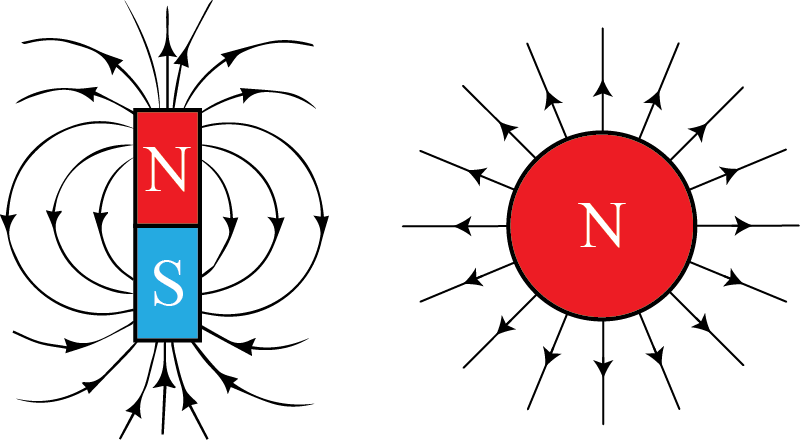
\includegraphics[width=0.7\textwidth]{assets/images/dipole-vs-monopole/dipole-vs-monopole.png}
  \caption[A magnetic dipole and monopole]
  {\label{fig:dipolemonopole}A magnetic dipole with North and South poles (left); a magnetic monopole, North pole only (right).  Image credit: \href{http://researchinschools.org}{Institute for Research in Schools}.}
\end{figure}
%

%=============================================================================
\subsection{The MoEDAL experiment}
\label{sec:moedalintro}
%=============================================================================
The \acf{MoEDAL}~\cite{MoEDAL2009}
%The Monopole and Exotics Detector at the LHC~\cite{MoEDAL2009}
is the latest and greatest in a long line of experiments which aims to
finally find evidence for the existence of magnetic monopoles.
%
It is designed to hunt for monopoles created in particle collisions
at the LHC using methods tailored to the strange properties of monopoles
and other highly-ionising particles.
As such it complements the searches for \ac{BSM} physics as performed by
the other LHC experiments,
providing another exciting way we can try to answer fundamental questions 
about our Universe.

%
\begin{figure}[htbp]
  \centering
  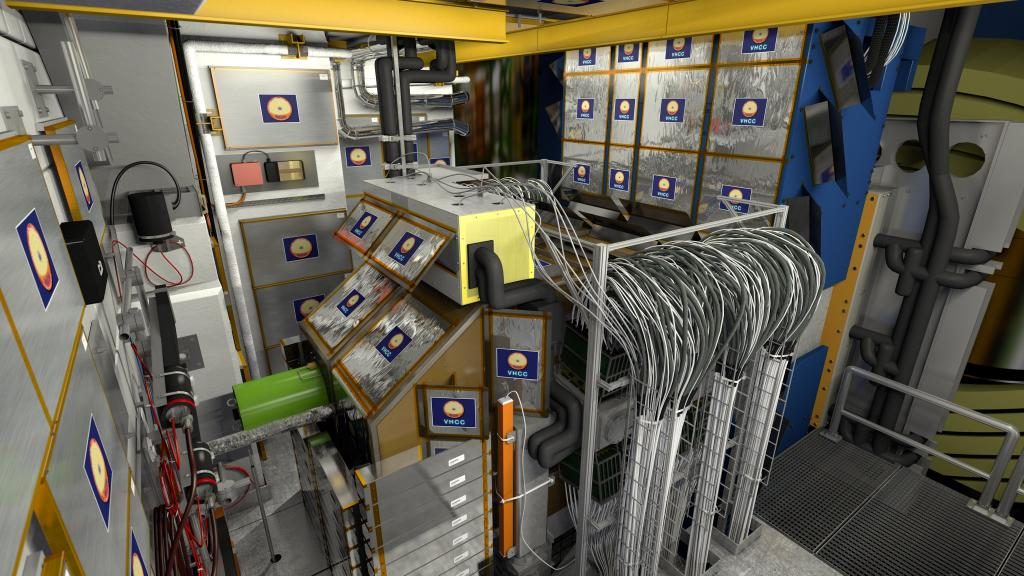
\includegraphics[width=0.9\textwidth]{assets/images/moedal-photo/moedal-photo.jpg}
  \caption[The MoEDAL experiment at CERN]
  {\label{fig:moedalphoto}The MoEDAL experiment at CERN.
Image credit: \href{http://moedal.web.cern.ch/}{The MoEDAL Collaboration};
please contact them regarding licensing/re-use of this image.}
\end{figure}
%

As we'll see,
one of these special techniques requires human input.
Many experiments can automate their searches for new physics using computer
programs because they use electronic readouts and are, generally speaking,
looking for well-understood particles.
%
The MoEDAL detector systems -- and the particles they are
looking for -- are very different,
and so require the human brain's enormous capability for image processing,
decision-making, and all-round ability to spot things that are ``odd''.
Which is where you come in -- MoEDAL needs your help!


%=============================================================================
\subsection{Overview of this guide}
\label{sec:overview}
%=============================================================================
Section~\ref{sec:theory} discusses the theory behind magnetic monopoles,
and presents a number of ideas that motivate the search for them.
The searches that have been carried out to-date are presented in
Section~\ref{sec:search}.
The MoEDAL experiment is described in more detail in
Section~\ref{sec:exp}, and finally the ways the reader may get involved
with MoEDAL is described in Section~\ref{sec:getinvolved}.


\clearpage

%%%%%%%%%%%%%%%%%%%%%%%%%%%%%%%%%%%%%%%%%%%%%%%%%%%%%%%%%%%%%%%%%%%%%%%%%%%%%%%
\section{The physics of magnetic monopoles}
\label{sec:theory}
%%%%%%%%%%%%%%%%%%%%%%%%%%%%%%%%%%%%%%%%%%%%%%%%%%%%%%%%%%%%%%%%%%%%%%%%%%%%%%%
To date there has been no solid, reproducible experimental evidence that
magnetic monopoles exist. For now, magnetic charge remains an entirely
theoretical concept that would, amongst other things, neaten up Maxwell's
equations of electrodynamics.
%
So why would we -- \emph{why should we} -- spend time and effort looking
for them? There are, in fact, some very good reasons to believe they exist
and that we just haven't found them yet.
%
One theorist has even said that they are ``\emph{one of the safest
bets one can make about physics not yet seen}''~\cite{Polchinski2004}.
%
In this section we look at some of these reasons -- so you
can decide for yourself!

%=============================================================================
\subsection{Dirac's magnetic monopole}
\label{sec:diracmonopole}
%=============================================================================
Paul Adrien Maurice Dirac (Figure~\ref{fig:pamdirac}) was a theoretical
theorist who played an important part in the development of quantum mechanics.
He was one of the first theoreticians to combine quantum mechanics with
special relativity with his eponymous equation~\cite{Dirac1928},
which allowed so-called ``negative energy'' solutions~\cite{Dirac1930}.
%
At first Dirac interpreted these solutions,
which would require the particle corresponding to the negatively-charged
electron to have a positive charge, as protons.
%
He noted in a subsequent paper~\cite{Dirac1931} that, actually,
the negative energy particles would need to have the same mass as the
electron -- the positively-charged anti-electron.
%
He had predicted antimatter.
%
This prediction was confirmed with Anderson's discovery of the
positron~\cite{Anderson1933} and the rest, as they say, is history.

%
\begin{figure}[htbp]
  \centering
  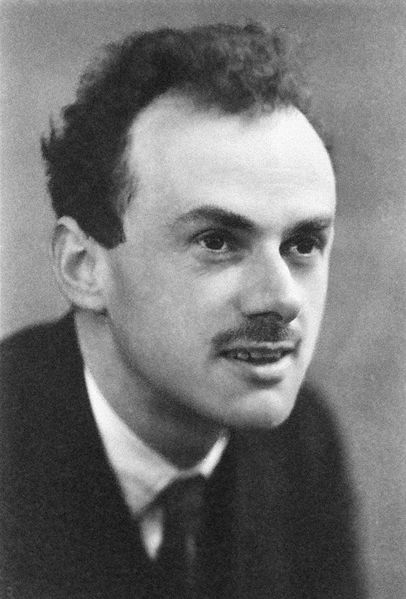
\includegraphics[width=0.25\textwidth]{assets/images/dirac-portrait/dirac-portrait.jpg}
  \caption[Paul A. M. Dirac]
  {\label{fig:pamdirac}%
Paul Adrien Maurice Dirac (1902-1984) predicted the existence of antimatter~\cite{Dirac1930}. %
Could he have been right about magnetic monopoles too?~\cite{Dirac1931}. %
Image credit: \href{https://commons.wikimedia.org/wiki/File:Dirac_4.jpg}{nobelprize.org} (public domain); %
please refer to their website regarding re-use of this image.} 
\end{figure}
%

Funnily enough, in the same paper Dirac had made another prediction.
(In fact, this prediction was the main point of the paper!)
In trying to explain why there was a smallest, discrete value of the
electric charge (i.e. why charge is quantised),
he postulated the existence of isolated magnetic charge that would show
a ``\emph{symmetry between electricity and magnetism quite foreign to current views}''.
He had predicted the magnetic monopole.

%
\begin{figure}[htbp]
  \centering
  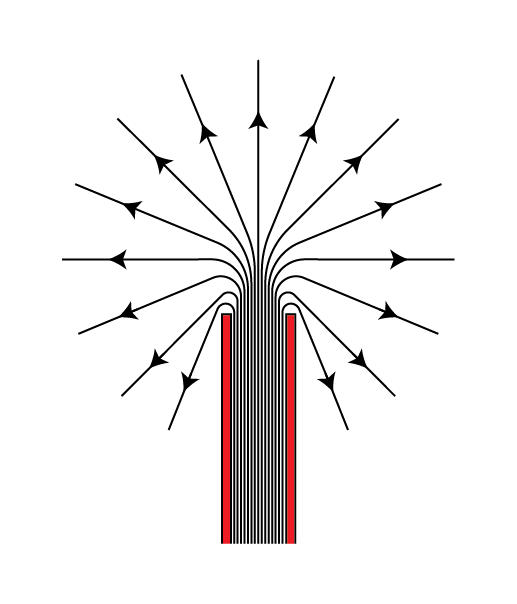
\includegraphics[width=0.5\textwidth]{assets/images/dirac-monopole/dirac-monopole.png}
  \caption[A schematic representation of Dirac's magnetic monopole]
  {\label{fig:diracmonopole}%
A schematic representation of Dirac's magnetic monopole.
The monopole is imagined to be the end point of a semi-infinitely long,
infinitesimally thin solenoid known as a ``Dirac string'',
here shown from the side (red lines).
%
The magnetic field lines (black arrows) are shown emanating from the point
at the end of the string (imagine the red lines are infinitely close together).
If such Dirac monopoles exist, it is the requirement that the string is
undetectable that means electric charge must be quantised.
%
Image credit: \href{http://researchinschools.org}{Institute for Research in Schools}.}
\end{figure}
%

Dirac's monopole was bit of a funny object.
Like a particle with electric charge,
the monopole would need to exude magnetic field field lines spherically
from its centre. Other magnetic charges placed in this field would experience
a force exactly analogous to the Coulomb force that pushes like charges apart
and pulls opposite charges together.
To create such a magnetic field configuration,
Dirac imagined a semi-infinitely long, infinitesimally thin solenoid
(i.e. a very, very tightly-wound coil with a flowing electric current).
%
The end of this ``Dirac string'' -- as shown schematically in
Figure~\ref{fig:diracmonopole} 2 -- represents the monopole.

While it is easy to imagine such a string,
one might not necessarily want to get tangled up in it.
Dirac showed that if such a string/monopole configuration did exist in
Nature, the only way that the mathematics could work out such that the
strings were undetectable by experiments was if electric charge was quantised.
There is an excellent explanation of the quantum theory behind this assertion
using the double slit experiment (as well as many other aspects of magnetic
monopoles) in~\cite{Rajantie2012}.
%
As the quantisation of charge is observed experimentally,
Dirac reasoned that magnetic monopoles (and their associated strings)
must exist.
%
Unfortunately, unlike the positron, monopoles were not found a few years
later.

%=============================================================================
\subsection{Grand Unified Theories}
\label{sec:guts}
%=============================================================================
Theorists, in the meantime, had been developing \ac{QFT}
as a way of describing matter and forces not in terms of particles or waves 
but mathematical constructs called fields.
%
(If you want to get your head around the wave-particle duality,
study physics at university and take a \ac{QFT} course.
Your hands will thank you from all of the ``hand-waving'' you won’t have to do.)
%
The 1960s saw the electromagnetic and weak forces -- two of the fundamental
forces of Nature -- united into a single electroweak force,
winning Glashow, Salam and Weinberg the 1979 Nobel Prize for
Physics.
The 1970s then saw a great deal of interest in literally going one
better -- uniting the electromagnetic, weak, and strong forces into one force.
Such a theory is known as a \ac{GUT}. %Grand Unified Theories (GUTs).
Figure~\ref{fig:forceunification} shows roughly where this ``Grand Unification''
might occur in terms of energy (around $10^{13}$ \ac{TeV}) and time
(about $10^{-36}$ seconds after the Big Bang).

%
\begin{figure}[htbp]
  \centering
  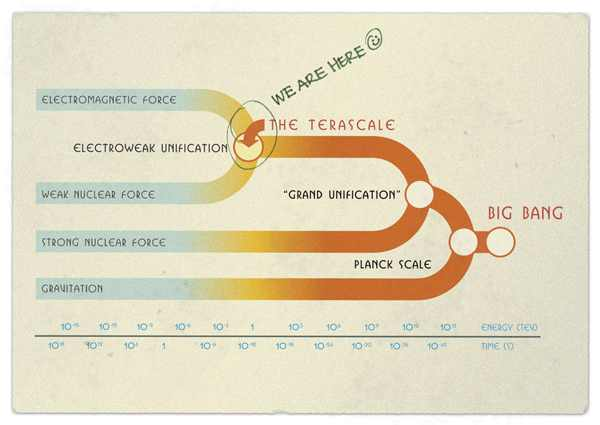
\includegraphics[width=0.6\textwidth]{assets/images/force-unification/force-unification.jpg}
  \caption[The unification of the four fundamental forces of Nature]
  {\label{fig:forceunification}%
The unification of the four fundamental forces of Nature,
as shown in this ``\emph{Postcard from the Terascale}''.
Image credit: Symmetry Magazine/Sandbox Illustrations; please contact them
regarding licensing/re-use of this image.}
\end{figure}
%

What does this have to do with magnetic monopoles?
Well, in the course of trying to get the mathematics to work,
two theorists independently found that an inevitable consequence of bringing
the three forces together was the appearance of terms in the equations that
represented particles (well, fields) with
magnetic charge~\cite{tHooft1974,Polyakov1974}.
You couldn't unite the strong force with the electroweak force
without magnetic monopoles\footnote{%
As it happens, the monopoles appear when you squeeze the \ac{GUT} to
quantise the electromagnetic field into particles.
So, as noted in many reviews of the magnetic monopole literature,
Dirac’s argument is reversed: the quantisation of the electromagnetic
field necessitates the existence of magnetic monopoles.}.
%
Of course, no Grand Unified Theory has been experimentally verified,
but if we believe in the ultimate unification of the
fundamental forces -- which, let’s be honest, would be rather nice -- it
turns out that we \emph{need} magnetic monopoles.

%=============================================================================
\subsection{Monopoles in the Standard Model}
\label{sec:smmonopole}
%=============================================================================
There is, however, one slight problem with \ac{GUT}-scale magnetic monopoles.
While one cannot predict the mass of the Dirac monopole,
\ac{GUT} monopole masses (which can be calculated) tend to be billions
and billions times the energies reachable by the \ac{LHC}, or indeed any
physical process occurring more than a fraction of a second after the Big Bang.
While we can look for ``relic'' monopoles in cosmic rays that reach the
Earth --and~\cite{Patrizii2015} provides an excellent summary of the searches
conducted so far -- we would need something between the Dirac monopole
and the \ac{GUT} monopole in order to have some hope of creating
magnetic monopoles in accelerators with all of the benefits that the
controlled conditions of the laboratory bring.

%
\begin{figure}[htbp]
  \centering
  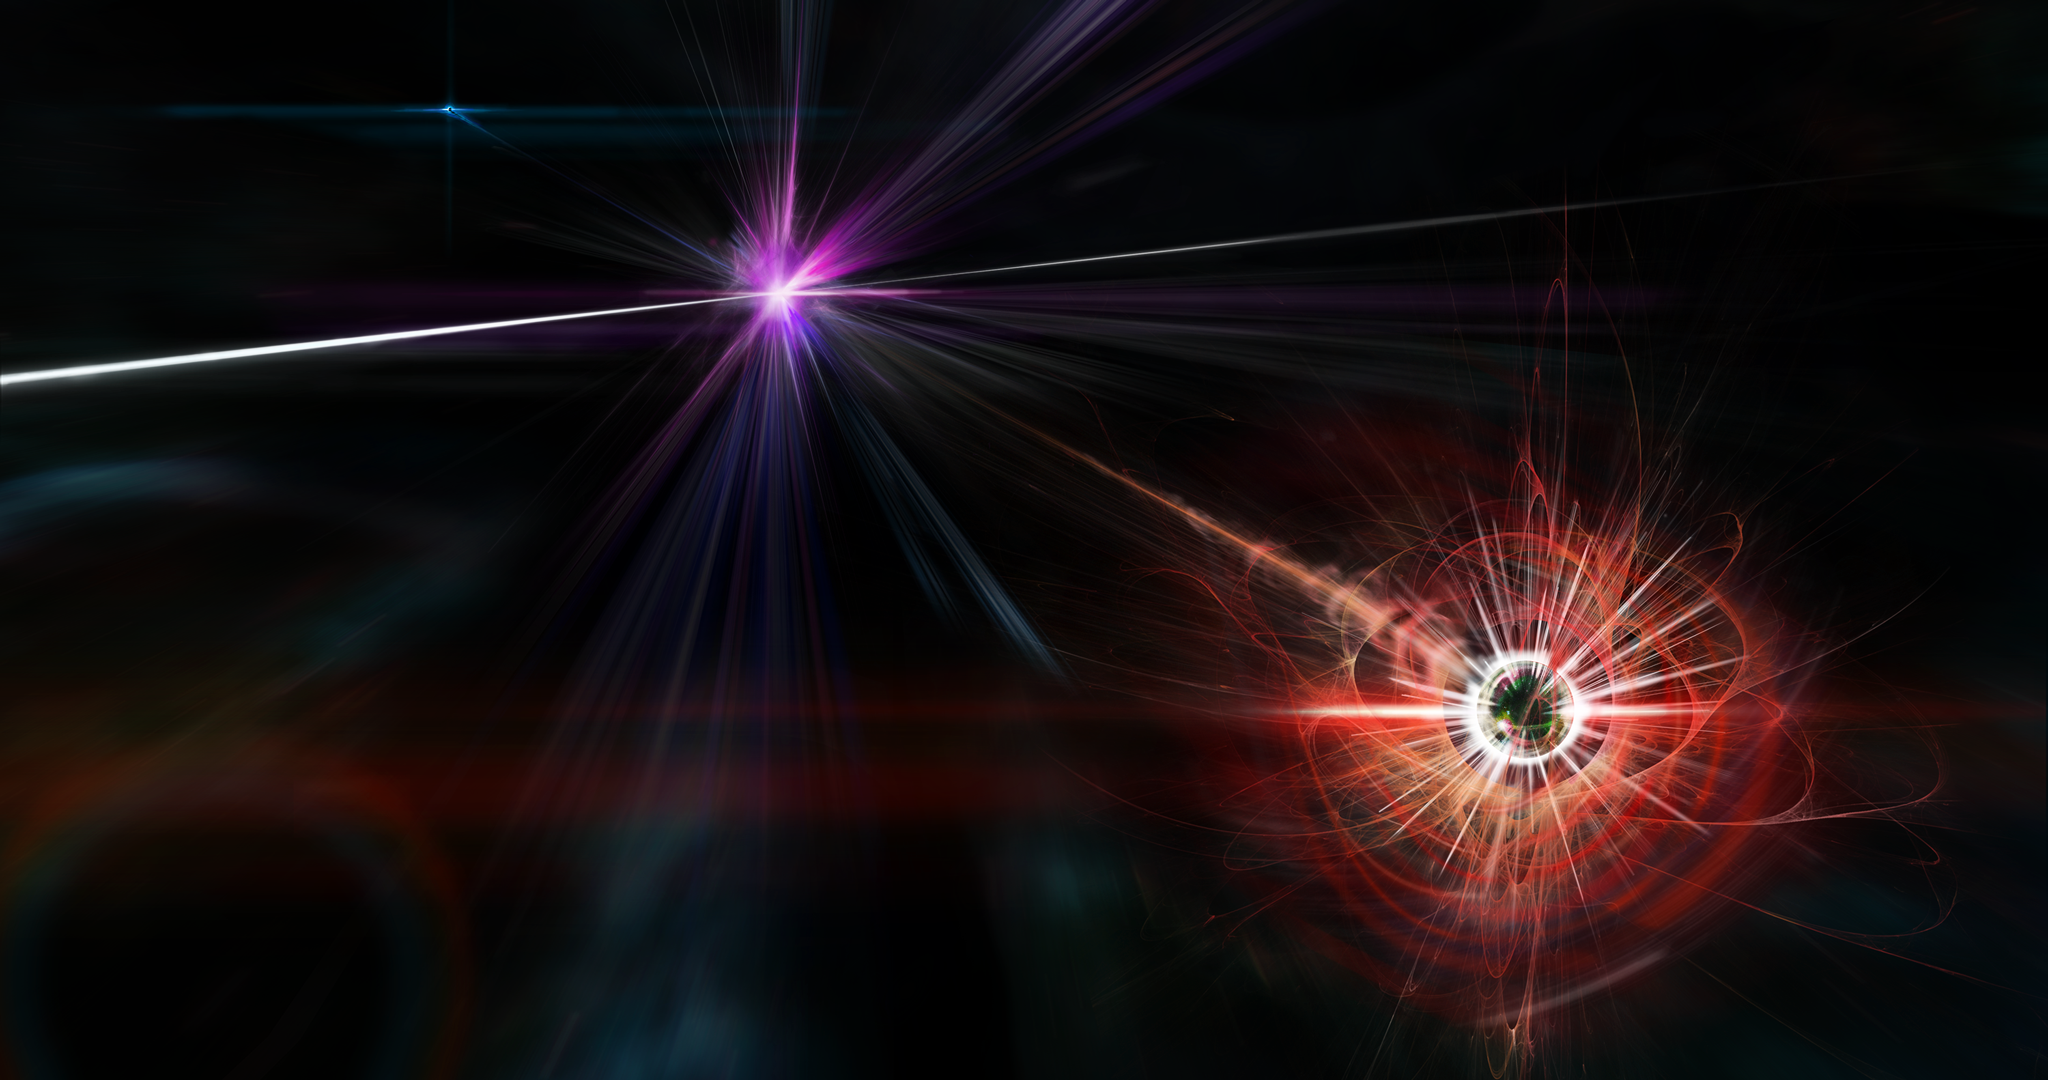
\includegraphics[width=1.0\textwidth]{assets/images/monopole-artist/monopole-artist.png}
  \caption[An artist's impression of magnetic monopole production at the LHC]
  {\label{fig:monopoleartist}%
An artist's impression of magnetic monopole production in a proton-proton
collision at the \acf{LHC}. Image credit: The MoEDAL Collaboration/H. Valja 2015;
please contact them regarding licensing/re-use of this image.}
\end{figure}
%

Fortunately, such a monopole has been proposed.
An ``\term{electroweak monopole}'' (which, incidentally, has twice the
magnetic charge of Dirac's monopole) can be made to appear in the
Standard Model of particle physics by adding some extra terms to the
field equations~\cite{Cho1997,Yang1998}.
In fact, the theorists behind the electroweak monopole insist that the
Standard Model is incomplete without the electroweak monopole -- and
given that we know the Standard Model is already broken
by the fact neutrinos have mass, we know that we can't just leave it at
the discovery of the Higgs boson.
%
Semantics aside, what's important is that some
recent papers~\cite{Kimm2016,Ellis2016} have suggested that the
electroweak monopole would have a mass of below 7 \acs{TeV},
putting it within tantalising reach of the Large Hadron Collider and
the MoEDAL experiment.
%
Figure~\ref{fig:monopoleartist} shows an artist's impression of
monopole-antimonopole production in \acs{LHC} proton-proton collisions.
%
The question is -- can Nature produce something as beautiful?


\clearpage

%%%%%%%%%%%%%%%%%%%%%%%%%%%%%%%%%%%%%%%%%%%%%%%%%%%%%%%%%%%%%%%%%%%%%%%%%%%%%%%
\section{The search for magnetic monopoles}
%\section{The search for magnetic monopoles (and other animals)}
\label{sec:search}
%%%%%%%%%%%%%%%%%%%%%%%%%%%%%%%%%%%%%%%%%%%%%%%%%%%%%%%%%%%%%%%%%%%%%%%%%%%%%%%
%%=============================================================================
%\subsection{The state of play}
%\label{sec:stateofplay}
%%=============================================================================
At the time of writing,
no experimental evidence for the existence of magnetic monopoles has been
recorded in the scientific literature.
While \ac{MoEDAL} hopes to change all of that with results from the \ac{LHC}'s
$13 \TeV$ proton-proton collisions, for now we can only look at the results
from all of the experiments that have tried so far.
These searches broadly fall into two categories:
looking for human-made monopoles from particle colliders (``farmed'')
and
looking for monopoles produced by Nature (``free-range'')
that would be found in cosmic rays that hit the Earth.

%
\begin{table}[htbp]
  \centering
  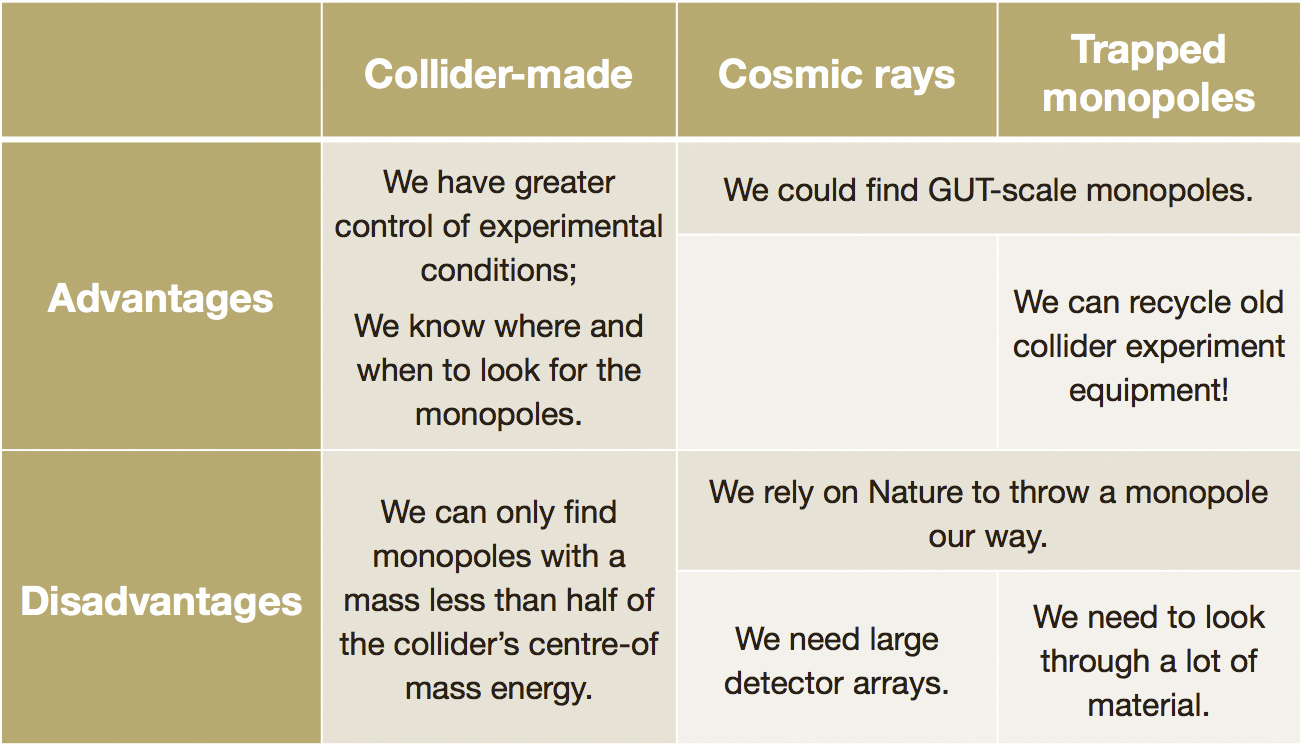
\includegraphics[width=0.75\textwidth]{assets/images/search-table/search-table.jpg}
  \caption[Monopole search strategies]
  {\label{tab:searchstrategies}The advantages and disadvantages of the different search %
strategies employed to find experimental evidence for magnetic monopoles.}
\end{table}
%

The advantage of the former approach is that we would know where and
(roughly) when the monopole-antimonopole pair was produced;
we have far more knowledge of the experimental conditions.
We are, however, limited by the centre-of-mass energy of the
collider in question.
Cosmic ray-based monopole searches rely on catching a ``free-range''
monopole by chance -- and the odds aren't great -- but are capable of
finding the sort of monopole required by \acp{GUT} which
are far beyond what colliders could ever hope to produce.

An excellent summary all the results to-date is presented in
Section 5 of L. Patrizii and M. Spurio’s review paper,
``{\em Status of Searches for Magnetic Monopoles}''~\cite{Patrizii2015}.
You can read the arXiv preprint of this paper
\href{http://arxiv.org/abs/1510.07125}{here}\footnote{%
See \href{http://arxiv.org/abs/1510.07125}{http://arxiv.org/abs/1510.07125}} for free.
The paper also contains sections on monopole theory,
energy losses, experimental methods and what the future holds for monopole
searches (including a shout-out to MoEDAL, of course!) -- so it's well worth
a read -- but some very brief summaries are provided below for convenience.


%=============================================================================
\subsection{Collider-based searches}
\label{sec:searchescollider}
%=============================================================================
{\em See Section 5.1 of~\cite{Patrizii2015} for further information and
full references.}

Magnetic monopoles have been looked for whenever a particle collider has
opened a new energy frontier.
For electron-positron collisions,
the latest results have come from experiments using the
\ac{LEP} collider (for which the LHC's tunnel was originally constructed).
%
\href{http://opal.web.cern.ch/Opal/}{OPAL} (see Figure~\ref{fig:opal})
and \acs{MODAL} (a forerunner of MoEDAL) experiments used both the active 
detector systems and \ac{NTD} arrays to spot monopole-antimonopole pairs.  
\acp{NTD} around beam interaction points were also used at the TRISTAN 
ring at \acs{KEK} (Japan), PETRA at DESY (Germany), and \acs{PEP} at
\acs{SLAC} (US).
Likewise, the best proton-antiproton results have come from Fermilab's
D0, \acs{CDF}, and FNAL E710 experiments using similar techniques.

%
\begin{figure}[htbp]
  \centering
  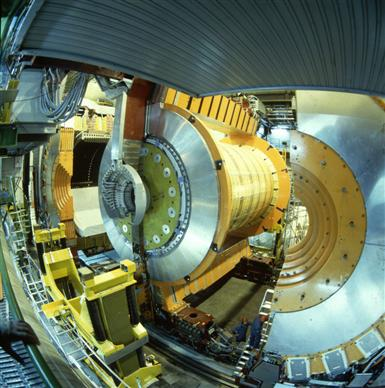
\includegraphics[width=0.6\textwidth]{assets/images/opal/opal.jpg}
  \caption[The OPAL experiment at CERN's LEP Collider]
  {\label{fig:opal}The \acf{OPAL} detector at Interaction Point 6 (IP6), %
which has set some of the most stringent limits on monopole production for %
electron-positron colliders. %
Image credit: \href{https://commons.wikimedia.org/wiki/File:OPAL.jpg}{CERN/Wikimedia Commons}; %
please refer to their terms of use regarding licensing/re-use of this image.}
\end{figure}
%

The best proton-proton results are from the \ac{LHC}'s \ac{ATLAS} and \ac{CMS}
detectors at 8 \ac{TeV}, though these are based on active (electronic) 
detectors. \ac{MoEDAL} will ultimately produce the best \ac{NTD}-based
searches for magnetic monopoles -- and you could part of this with \ac{IRIS}!

%=============================================================================
\subsection{Cosmic ray-based searches}
\label{sec:searchescosmicray}
%=============================================================================
{\em See Sections 5.2 and 5.3 of~\cite{Patrizii2015} for further
information and full references.}

Searches for monopoles in cosmic rays typically need to take place in 
underground laboratories, where backgrounds from cosmic muons or background 
radiation can be minimised.
The best results so far come from the \acf{MACRO} observatory at the
Laboratori Nazionali del Gran Sasso, Italy (Figure~\ref{fig:macro}).
%
Using a combination of liquid scintillation detectors, streamer tubes, 
and \acfp{NTD} -- the largest ever deployed -- \ac{MACRO} saw only
ever saw a ``dummy'' monopole event (used to test the detection systems).
It completed its experimental run in 2001.

%
\begin{figure}[htbp]
  \centering
  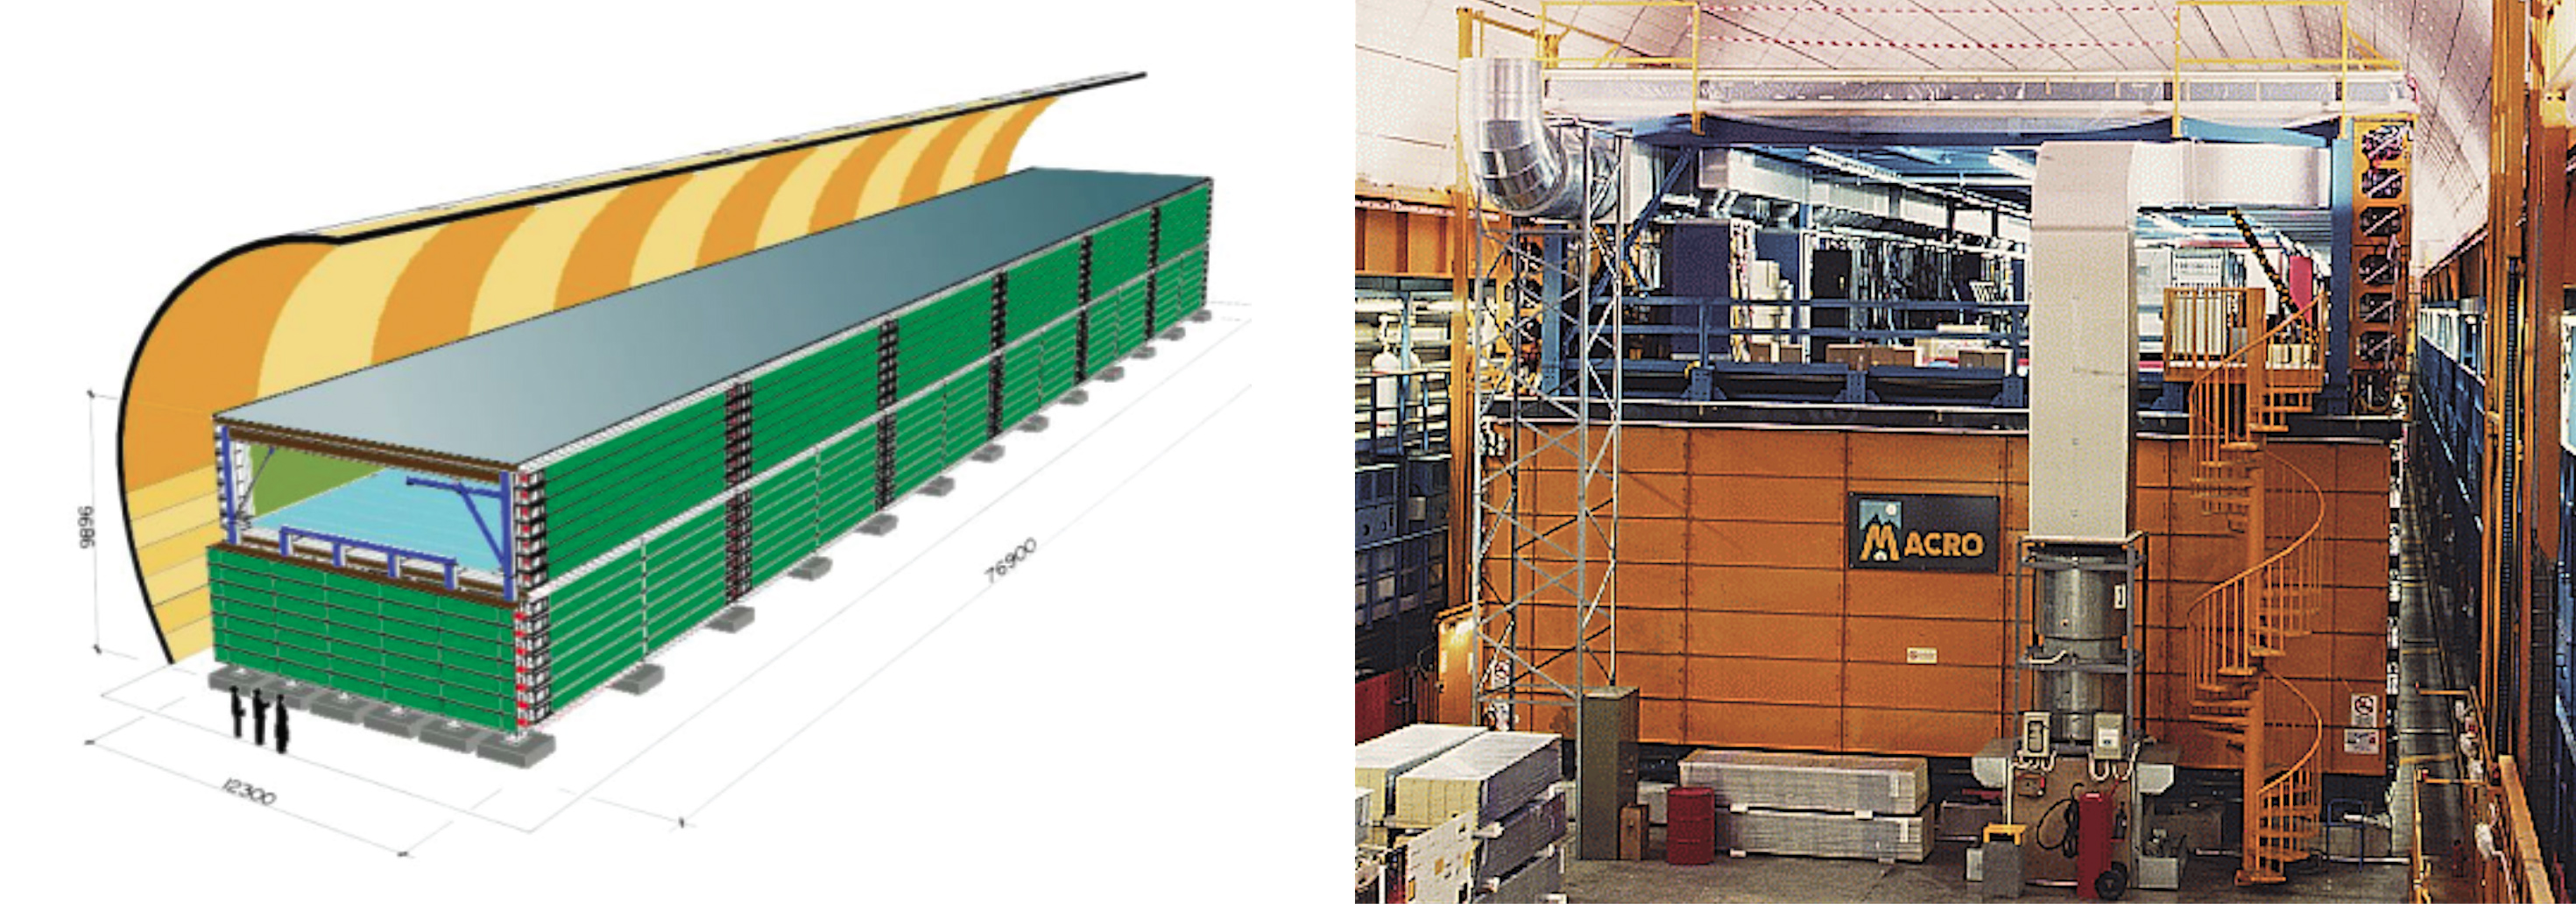
\includegraphics[width=1.0\textwidth]{assets/images/macro/macro.jpg}
  \caption[The MACRO experiment]
  {\label{fig:macro}The \acs{MACRO} (Monopole, Astrophysics and Cosmic Ray) %
observatory at the Laboratori Nazionali del Gran Sasso, Italy. %
Left -- artist's impression; %
right -- the detector itself. %
Image credit: \href{http://arxiv.org/abs/0707.1691}{The MACRO Collaboration}; %
please contact them regarding licensing/re-use of this image.}
\end{figure}
%

If cosmic ray backgrounds can be accounted for, other types of searches 
are possible.  The \ac{SLIM} experiment (Figure~\ref{fig:slim}) used
\acp{NTD} at an altitude of 5.2km exposed for just over four years.
Searches for relativistic monopoles have been conducted with neutrino 
telescopes like \acs{AMANDA}, \acs{ANTARES}, and IceCube 
(See Section 5.2.2 of~\cite{Patrizii2015} for more information).
These rely on the huge showers of Cerenkov light that monopoles would 
produce in the Antarctic ice, but due to the cosmic backgrounds can only 
look for candidates have come up all the way through the Earth.  
Again, these have seen nothing and the best result remains that of the 
\ac{MACRO} experiment.

%
\begin{figure}[htbp]
  \centering
  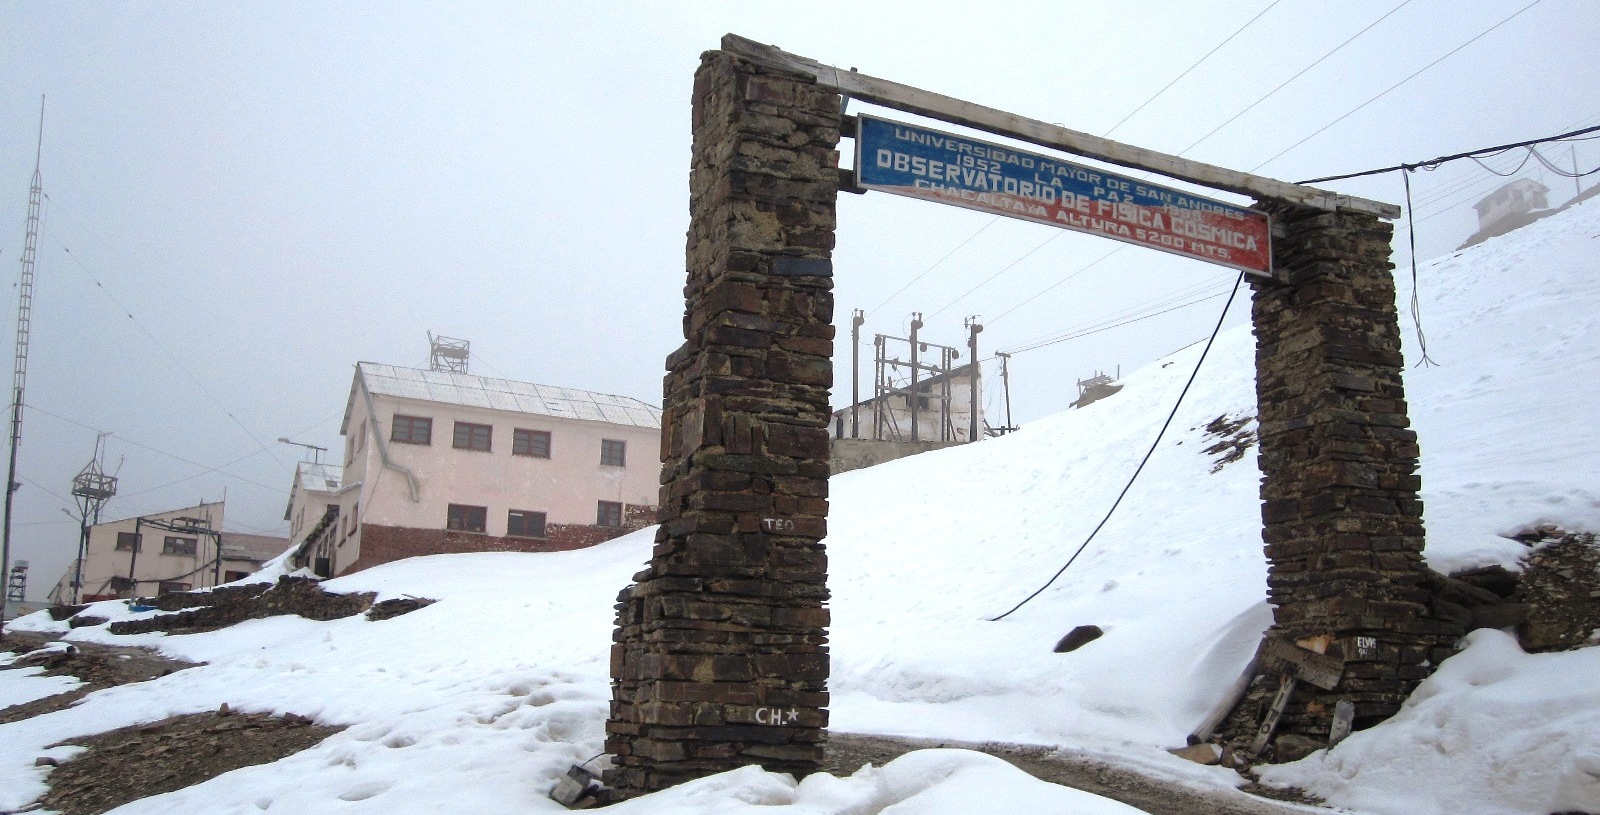
\includegraphics[width=1.0\textwidth]{assets/images/slim/slim.jpg}
  \caption[The Chacaltaya Astrophysical Observatory]
  {\label{fig:slim}The Chacaltaya Astrophysical Observatory, home of the %
\acs{SLIM} (Search for LIght magnetic Monopoles) experiment~\cite{SLIM2008a, SLIM2008b} %
which looked for magnetic monopoles in cosmic rays at an altitude of 5,230m above sea level. %
Image credit: \href{https://commons.wikimedia.org/wiki/File:Chacaltaya\_Astrophysical\_Observatory\_\%2804\%29.JPG}{Wikimedia Commons}; %
please refer to their terms of use them regarding licensing/re-use of this image.}
\end{figure}
%


%=============================================================================
\subsection{Trapped monopoles}
\label{sec:searchestrapped}
%=============================================================================
{\em See Sections 5.1 and 5.4 of~\cite{Patrizii2015} for further information
and full references.}

The third category of search takes a slightly different approach. 
Rather than record the tracks left by a magnetic monopole, 
one can try looking for monopoles in sample of material that might slow down 
a monopole enough to stop it and trap it.  
The trick is picking the right material, but the technique can be applied 
to both collider-produced and cosmic ray monopoles.  
For example, the H1 experiment at \acs{DESY}, Germany cut up 60cm of its 
aluminium beam pipe into pieces and scanned them with a \acf{SQUID}
to look for magnetic monopoles produced in the electron-proton collisions 
of \acs{HERA} (see Figure~\ref{fig:h1}).
Likewise, work has been carried out with material from the D0 and \acs{CDF}-based
Tevatron experiments (i.e. proton-antiproton collisions). 
Cosmic (i.e. \ac{GUT}-scale) monopoles have been looked for in terrestrial, 
lunar and meteoric material using similar methods.

%
\begin{figure}[htbp]
  \centering
  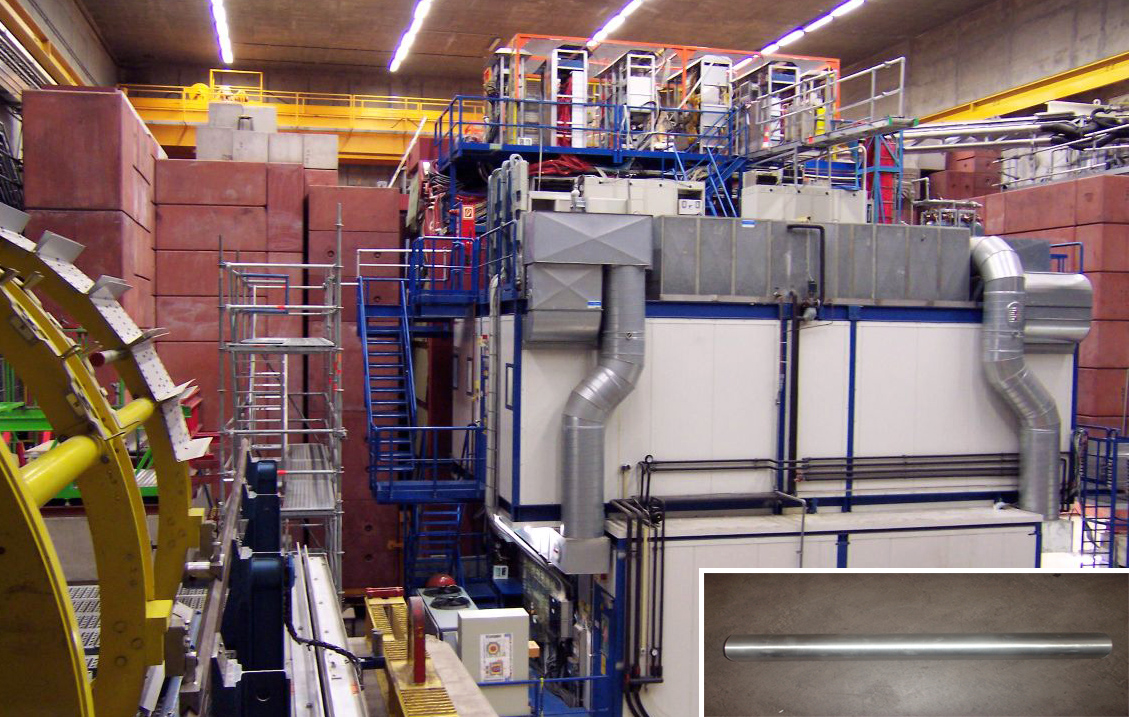
\includegraphics[width=1.0\textwidth]{assets/images/h1/h1.jpg}
  \caption[The H1 detector at DESY, Germany]
  {\label{fig:h1}The H1 detector at \ac{DESY}, Germany. %
Inset (bottom-right): a 60cm section of the H1 beam pipe used between 1994 %
and 1997 in a trapped monopole search. %
Image credit: \href{https://en.wikipedia.org/wiki/File:H1\_detector.jpg}{G. Brandt/Wikimedia Commons}; %
please refer to their terms of use regarding licensing/re-use of this image.}
\end{figure}
%

\ac{MoEDAL} continues this tradition with its \acf{MMT} subdetector (Section~\ref{sec:mmt}), 
which consists of hundreds of kilograms of aluminium bars placed within the \acs{LHCb} cavern.
These can then be removed and replaced during the \ac{LHC} shutdowns to allow \acs{SQUID}
scans of the bars to be made before the \ac{LHC} finishes running and the \ac{ATLAS} and \ac{CMS}
detectors are decommissioned.


\clearpage

%%%%%%%%%%%%%%%%%%%%%%%%%%%%%%%%%%%%%%%%%%%%%%%%%%%%%%%%%%%%%%%%%%%%%%%%%%%%%%%
\section{The MoEDAL experiment at CERN}
\label{sec:exp}
%%%%%%%%%%%%%%%%%%%%%%%%%%%%%%%%%%%%%%%%%%%%%%%%%%%%%%%%%%%%%%%%%%%%%%%%%%%%%%%
%%=============================================================================
%\subsection{The LHC's magnificent seventh}
%\label{sec:moedalexpintro}
%%=============================================================================
In December 2009, the CERN Research Board approved the
\acs{LHC}'s seventh experiment -- the
Monopole and Exotics Detector at the LHC,
also known as \acs{MoEDAL}~\cite{MoEDAL2009}.
%
Housed in the same underground cavern as
the \acs{LHCb}~\cite{LHCb2008} experiment at
Interaction Point 8 (see Figure~\ref{fig:moedallhcbsim}),
\ac{MoEDAL} continues the collider-based search for magnetic monopoles
at today's particle physics energy frontier:
the proton-proton collisions of the \ac{LHC}.
Like all \ac{LHC} experiments,
the scientific work -- installing and running the detectors,
processing the data, and publishing the results -- is done by the
\ac{MoEDAL} Collaboration.
\acs{IRIS} is a member of the \ac{MoEDAL} Collaboration,
and so -- by being a member of \ac{IRIS} -- you are too!

%
\begin{figure}[htbp]
  \centering
  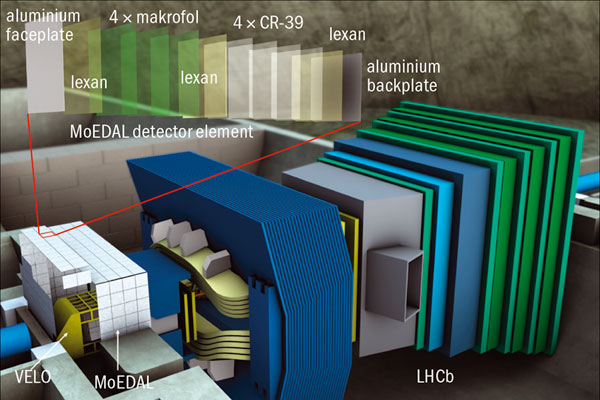
\includegraphics[width=1.0\textwidth]{assets/images/moedallhcbsim/moedallhcbsim.jpg}
  \caption[The MoEDAL experiment in the LHCb cavern]
  {\label{fig:moedallhcbsim}The \ac{MoEDAL} experiment in the \ac{LHCb} %
cavern, with the \ac{LHCb} detector (and \ac{VeLo} subdetector) shown for %
context.  The structure of a \ac{MoEDAL} \acf{NTD} element is shown %
in the exploded inset image. Image credit: \href{http://moedal.web.cern.ch}{The MoEDAL Collaboration}; %
please contact them regarding licensing/re-use of this image.}
\end{figure}
%

The first test detector elements of the \ac{MoEDAL} experiments were
installed in 2009, just before the \ac{LHC} was restarted following its
2008 malfunction.
%
The first full stack of Nuclear Track Detectors (NTDs – see below) were
put in place in January 2011, and officially began taking data on the
3rd of June 2015.
%
Since the publication of the \ac{MoEDAL} \ac{TDR} in 2009~\cite{MoEDAL2009},
however, the \ac{MoEDAL} experiment has grown and evolved to incorporate
additional subdetector systems to improve the chances of discovering a
magnetic monopole (or sign of physics beyond the Standard Model).
Let's take a look at these now.

%%=============================================================================
%\subsection{The subdetector systems}
%\label{sec:moedalsubdet}
%%=============================================================================

%-----------------------------------------------------------------------------
\subsection{The Nuclear Track Detectors}
\label{sec:ntds}
%-----------------------------------------------------------------------------
The \ac{MoEDAL} design concept was initially based only on the use of
devices known as \acfp{NTD}, following in the footsteps of the last monopole
searches carried out in CERN's 27km underground tunnel~\cite{Pinfold2009}.
\acp{NTD} are essentially sheets of material that, when hit with a massive,
highly-ionizing particle (\acs{HIP}), get damaged in such a way that we can 
analyse the damage and infer properties of whatever caused it.
%
For example, in the CR-39 \textregistered{} plastic used by \ac{MoEDAL},
\acp{HIP} break bonds in the plastic's hydrocarbons along the path of
the \ac{HIP}.
%
Careful etching with sodium hydroxide (NaOH) forms conical pits in the 
surface of the plastic along these paths, and by analysing the size, 
shape and angle of the cones we can learn more about the particle that 
caused them. \ac{MoEDAL} uses four types of \ac{NTD} material:
Lexan, Makrofol, and CR-39~\textregistered, each of which have different
sensitivities to the \ac{HIP}'s charge and momentum.
These can be seen in the exploded inset image in Figure~\ref{fig:moedallhcbsim}
(schematic) and the top-left of Figure~\ref{fig:ntd} (actual sheets).
Recently, additional sheets of Makrofol have been added within the \ac{LHCb}
experiment itself in the form of the \ac{VHCC} in order to increase the 
chances of spotting a monopole.

%
\begin{figure}[htbp]
  \centering
  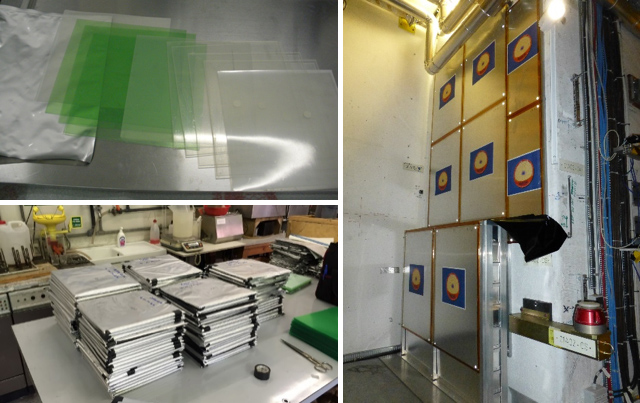
\includegraphics[width=1.0\textwidth]{assets/images/ntd/ntd.jpg}
  \caption[The MoEDAL Nuclear Track Detectors]
  {\label{fig:ntd}The component sheets of a MoEDAL \acf{NTD} stack (top-left); %
\ac{MoEDAL} \ac{NTD} stacks ready for deployment in the \ac{LHCb} cavern (bottom-left), %
and; some of the \ac{MoEDAL} \acp{NTD} in situ (right).  %
Image credit: \href{http://moedal.web.cern.ch}{R. Soluk/The MoEDAL Collaboration}; please contact them regarding licensing/re-use of this image.}
\end{figure}
%

In many ways, \acp{NTD} are like the nuclear emulsions used by particle
physicists in the 1950s in cosmic ray and early accelerator experiments.
The use of such emulsions was pioneered by Cecil Powell,
who won the 1950 Nobel Prize for Physics for this technique and the
discoveries he made with it.
%
The passage of a charged particle through the emulsion would ionise the
sensitive particles in such a way that the application of a chemical
would produce a light-blocking substance along the path,
making it visible.
The same principle is used in film-based photography.
The key thing is the sensitivity of the particles in the emulsion;
Powell's silver iodide-based emulsions were great for discovering mesons
in balloon flights or up mountains,
but would be overwhelmed by the energy and intensity of what the
LHC's collisions produce.

Luckily, magnetic monopoles are predicted to be so highly-charged
that we can use something less sensitive, more stable, and a bit cheaper
to record the tracks they would leave behind.
While breaking hydrocarbon bonds in a plastic is a different physical process,
the principles are the same -- including those used in the analysis.
Terabytes of digital images of the etched plastic from \ac{MoEDAL} \ac{NTD}
stacks -- like those shown in Figure~\ref{fig:ntd} -- need to be checked
for the tell-tale tracks of the monopole.
Given the unknown nature of the signal we expect (and the complexity of the
proton-proton collision background),
we will need help to do this -- which is one of the ways you can help.

%-----------------------------------------------------------------------------
\subsection{The Magnetic Monopole Trapper}
\label{sec:mmt}
%-----------------------------------------------------------------------------
The \acf{MMT} goes one step further than the \acfp{NTD}.
Rather than just recording the passage of the monopole through the material --
like finding the footprints of an animal in the jungle -- the \acp{MMT}
literally aim to trap the monopole so that it can be taken away and
studied further.
The \ac{MMT} is made up of many bars of aluminium packed closely 
together in boxes that are put in the \ac{LHCb} cavern around the
Interaction Point (see Figure~\ref{fig:mmt}).
If we're lucky, magnetic monopoles passing through the aluminium would
slow down, stop, and become trapped within the aluminium. We can then 
carefully remove the bars from the cavern and pass them through a \acf{SQUID},
which would detect the monopole's magnetic charge~\cite{Mermod2014}.

%
\begin{figure}[htbp]
  \centering
  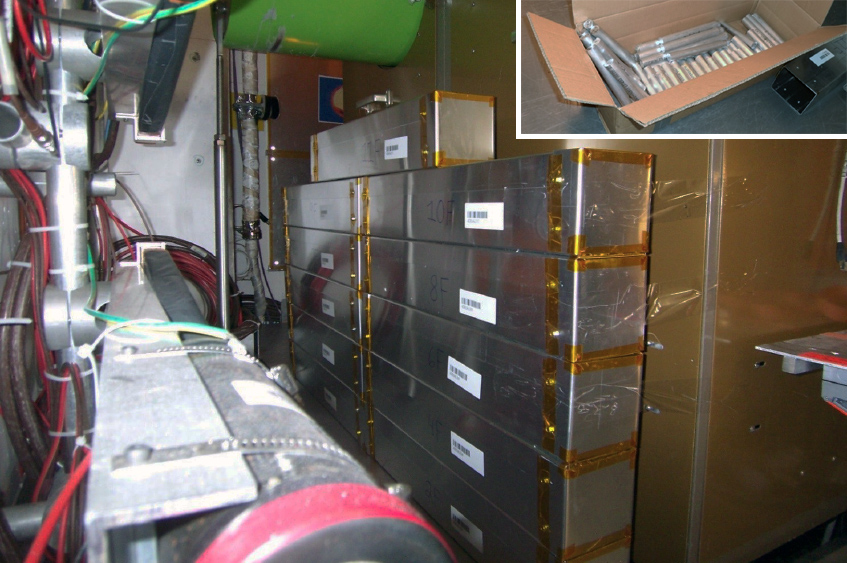
\includegraphics[width=1.0\textwidth]{assets/images/mmt/mmt.jpg}
  \caption[The MoEDAL Magnetic Monopole Trapper]
  {\label{fig:mmt}MoEDAL's prototype \acf{MMT} installed in the \ac{LHCb} cavern. %
Each box contains several bars of aluminium (see inset image, top-right) %
that are later removed from the cavern and scanned using a \ac{SQUID} %
to identify trapped magnetic monopoles.  %
Image credit: \href{http://moedal.web.cern.ch}{R. Soluk/The MoEDAL Collaboration}; %
please contact them regarding licensing/re-use of this image.}
\end{figure}
%

Finding a monopole this way would be particularly exciting,
as with the monopole embedded in the material of the detector we would 
have the chance to perform all sorts of studies to find out more about the 
properties of magnetic monopoles.  In fact, searches for trapped monopoles 
from collider experiments have been performed before using decommissioned detector 
and beam pipe elements.  The beauty of MoEDAL's \acp{MMT} is that they 
are purpose-built for monopole trapping, and we don't have to wait for \acs{CMS}
and \acs{ATLAS} to finish their work and throw their kit away!

%-----------------------------------------------------------------------------
\subsection{The MoEDAL Timepix array}
\label{sec:timepixarray}
%-----------------------------------------------------------------------------
The particle collisions that take place during \ac{LHC} running -- with both
protons and lead ions -- produce a great deal of ionising radiation.
For the general-purpose \ac{LHC} experiments,
much of this is uninteresting in the sense that we understand its properties 
and studying it further will (generally speaking) not lead to new discoveries.
Signatures from these particles is known as ``background'' to the signal 
and needs to be filtered out from the data.
The \ac{MoEDAL} \acp{NTD} and \acp{MMT} are only sensitive to highly-ionising 
particles (\acp{HIP}) like monopoles, and so in principle do not need to 
worry about this background.
%
That said, it is important to double-check this assertion by measuring 
the background radiation in the \acs{LHCb} cavern. To this end, a number 
of Timepix hybrid silicon pixel detectors~\cite{Timepix2007, Timepix2008Erratum}
have been installed in the vicinity of \acs{LHCb}'s \acf{VeLo}.
The location of each device is shown in Figure~\ref{fig:tpx}.
\acs{IRIS} has access to data from these detectors -- which are of course the same 
detectors as used in the CERN@school detector network, LUCID, and the 
\acf{ISS}. Discovering something like a magnetic monopole would be an 
extraordinary discovery, and so demonstrating that we understand any possible 
backgrounds would be an essential part of verifying the discovery.
% before we 
%all get on the plane to Stockholm.

%
\begin{figure}[htbp]
  \centering
  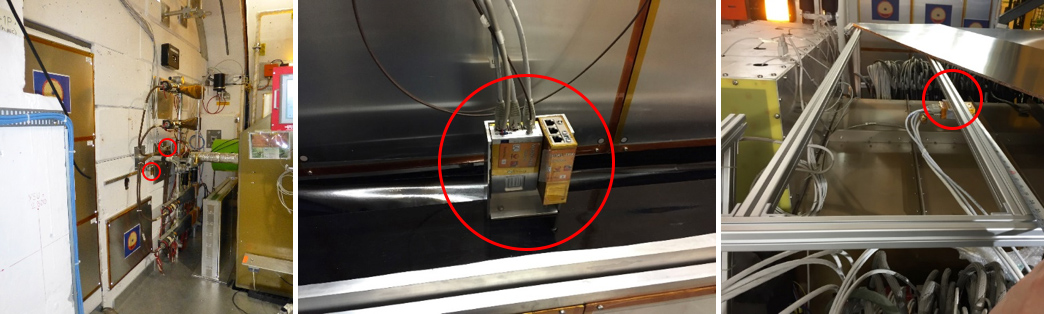
\includegraphics[width=1.0\textwidth]{assets/images/tpx/tpx.jpg}
  \caption[The MoEDAL Timepix detector array]
  {\label{fig:tpx}MoEDAL's five Timepix devices deployed around the %
\acs{LHCb} \acs{VeLo}. In the left-most image, TPX2 (TPX4) is shown %
in the lower-left (upper-right) red circle, where it has been installed %
with the sensor plane normal (parallel) to the beam pipe. %
In the central image, TPX1 (TPX3) is shown on the left (right) where it %
has been installed on the side of the \acs{VeLo} enclosure with the sensor %
plane normal (parallel) to the beam pipe. In the right-most image, TPX5 %
is shown installed above the \acs{VeLo} enclosure with the sensor plane %
normal to the beam pipe. %
Image credit: \href{http://moedal.web.cern.ch}{R. Soluk/The MoEDAL Collaboration}; %
please contact them regarding licensing/re-use of this image.}
\end{figure}


\clearpage

%%%%%%%%%%%%%%%%%%%%%%%%%%%%%%%%%%%%%%%%%%%%%%%%%%%%%%%%%%%%%%%%%%%%%%%%%%%%%%%
\section{Get involved!}
\label{sec:getinvolved}
%%%%%%%%%%%%%%%%%%%%%%%%%%%%%%%%%%%%%%%%%%%%%%%%%%%%%%%%%%%%%%%%%%%%%%%%%%%%%%%
So you want to help look for magnetic monopoles at the Large Hadron Collider?
Great! This section will take you through what you need to do, how to do it,
and how to get help if you need it.

%=============================================================================
\subsection{Getting started}
\label{sec:zooniversegettingstarted}
%=============================================================================
In order to give you access to the MoEDAL experiment data,
and tools you'll need to analyse it, the Institute for Research in Schools
has called in some help from our friends at the
\href{http://www.zooniverse.org}{Zooniverse}.
The Zooniverse started with the
\href{http://www.galaxyzoo.org}{Galaxy Zoo} project,
where people were invited to classify thousands of images of galaxies from
the Sloan Digital Sky Survey.
It has since evolved into the world's largest and most popular platform
for people-powered research that has led to peer-reviewed publications
and opened the door to many new areas of scientific research that just
would not be possible otherwise.
MoEDAL has created the Monopole Quest! project within the Zooniverse,
and by taking part in this you'll be joining the millions of Zooniverse
volunteers helping to do
\href{https://www.zooniverse.org/about/publications}{real science}.

%-----------------------------------------------------------------------------
\subsubsection{Creating a Zooniverse account}
\label{sec:zooniverseaccount}
%-----------------------------------------------------------------------------
The first thing to do is to visit the Zooniverse website\footnote{%
See \href{http://www.zooniverse.org}{http://www.zooniverse.org}}
and create a user account.
%
You can do this on a desktop computer, a laptop, a tablet or even a
smartphone (if the screen is big enough!).
If you're a student, you may wish to ask your teacher to do this for you
or for them to create an account for your class.
You don't have to create an account to take part in Monopole Quest!,
but in order for your work to be credited you need to be logged in.
Always ask your teacher or your IRIS contact for advice if you need to.
Creating a user account is simple -- you can create a user account by
filling in the online form you get when you click on the ``Register''
link at the top-right of the Zooniverse homepage.

%-----------------------------------------------------------------------------
\subsubsection{Sign in and access the Monopole Quest! project}
\label{sec:zooniversesignin}
%-----------------------------------------------------------------------------
Once you have created an account,
sign in to the Zooniverse by clicking the ``Sign in'' link
(also at the top-right of the homepage).
Then you can access the Monopole Quest! project at the following URL:

\begin{itemize}
\item \url{https://www.zooniverse.org/projects/twhyntie/monopole-quest}
\end{itemize}

After which you should see the Monopole Quest! landing page as
shown in Figure~\ref{fig:mqlandingpage}.

%
\begin{figure}[htbp]
  \centering
  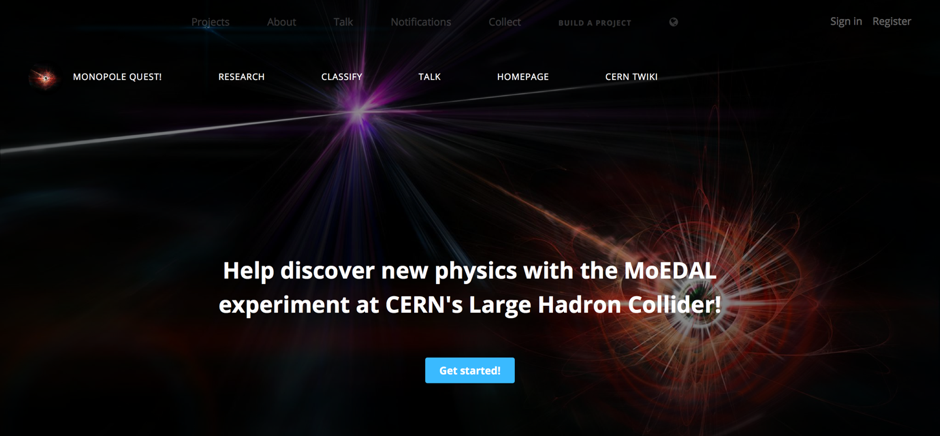
\includegraphics[width=1.0\textwidth]{assets/images/mqlandingpage/mqlandingpage.png}
  \caption[The Monopole Quest! project landing page]
  {\label{fig:mqlandingpage}The Monopole Quest! landing page on the Zooniverse.
From here you can get stuck into some real MoEDAL data straight away!}
\end{figure}
%

Then click on the ``Get started!'' button and start doing some science!

%=============================================================================
\subsection{The Monopole Quest! project}
\label{sec:monopolequest}
%=============================================================================

%-----------------------------------------------------------------------------
\subsubsection{What do I do?}
\label{sec:mqwhatdoido}
%-----------------------------------------------------------------------------
As with all Zooniverse projects, Monopole Quest! will ask you a number of
questions about an image from one or more their datasets.
Your answers to these questions will result in a classification for that
image -- information about that data that will help scientists with
some aspect of the research.
For example, the first question in Monopole Quest! asks you if you can
see any ``blobs'' in the image (see Figure~\ref{fig:mqblobq}).
These blobs correspond to the etched pits in the
\ac{NTD} scans that may be caused by monopoles or other \acp{HIP}.
So, in essence, you are being asked if you can see any potential
monopole signals!

You can answer the questions by selecting the appropriate answer with your
mouse (or tapping the option on a touch screen) and then pressing the
``Done'' button.
You'll then be asked the next question or asked to perform a task,
such as drawing a shape on the image.
For example, if you can see a blob in the image, you'll be asked to draw
around it with a circle (the ``blob marking tool'') in order to measure
its size (see Figure~\ref{fig:mqdrawing}).

%
\begin{figure}[p]
  \centering
  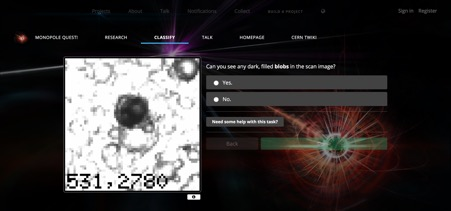
\includegraphics[width=0.8\textwidth]{assets/images/mqblobq/mqblobq.jpg}
  \caption[Monopole Quest! Can you see any blobs?]
  {\label{fig:mqblobq}The first question from the Monopole Quest!
Zooniverse project (Jan. 2017).}
\end{figure}
%

%
\begin{figure}[p]
  \centering
  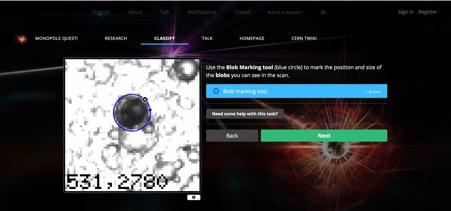
\includegraphics[width=0.8\textwidth]{assets/images/mqdrawing/mqdrawing.jpg}
  \caption[Monopole Quest! An example drawing task]
  {\label{fig:mqdrawing}An example drawing task in the Monopole Quest! project
(Jan. 2017).}
\end{figure}
%

%-----------------------------------------------------------------------------
\subsubsection{How do I get help?}
\label{sec:mqhelp}
%-----------------------------------------------------------------------------
As there are many questions and tasks to do in Monopole Quest!,
we have added interactive help to the questions themselves rather than
list everything here.  If you need help at any point, click on the
``Need some help with this task?'' button and a pop-up window will appear
that will give you some additional guidance if you get stuck.
Figure~\ref{fig:mqhelp} shows an example of this.

%
\begin{figure}[htbp]
  \centering
  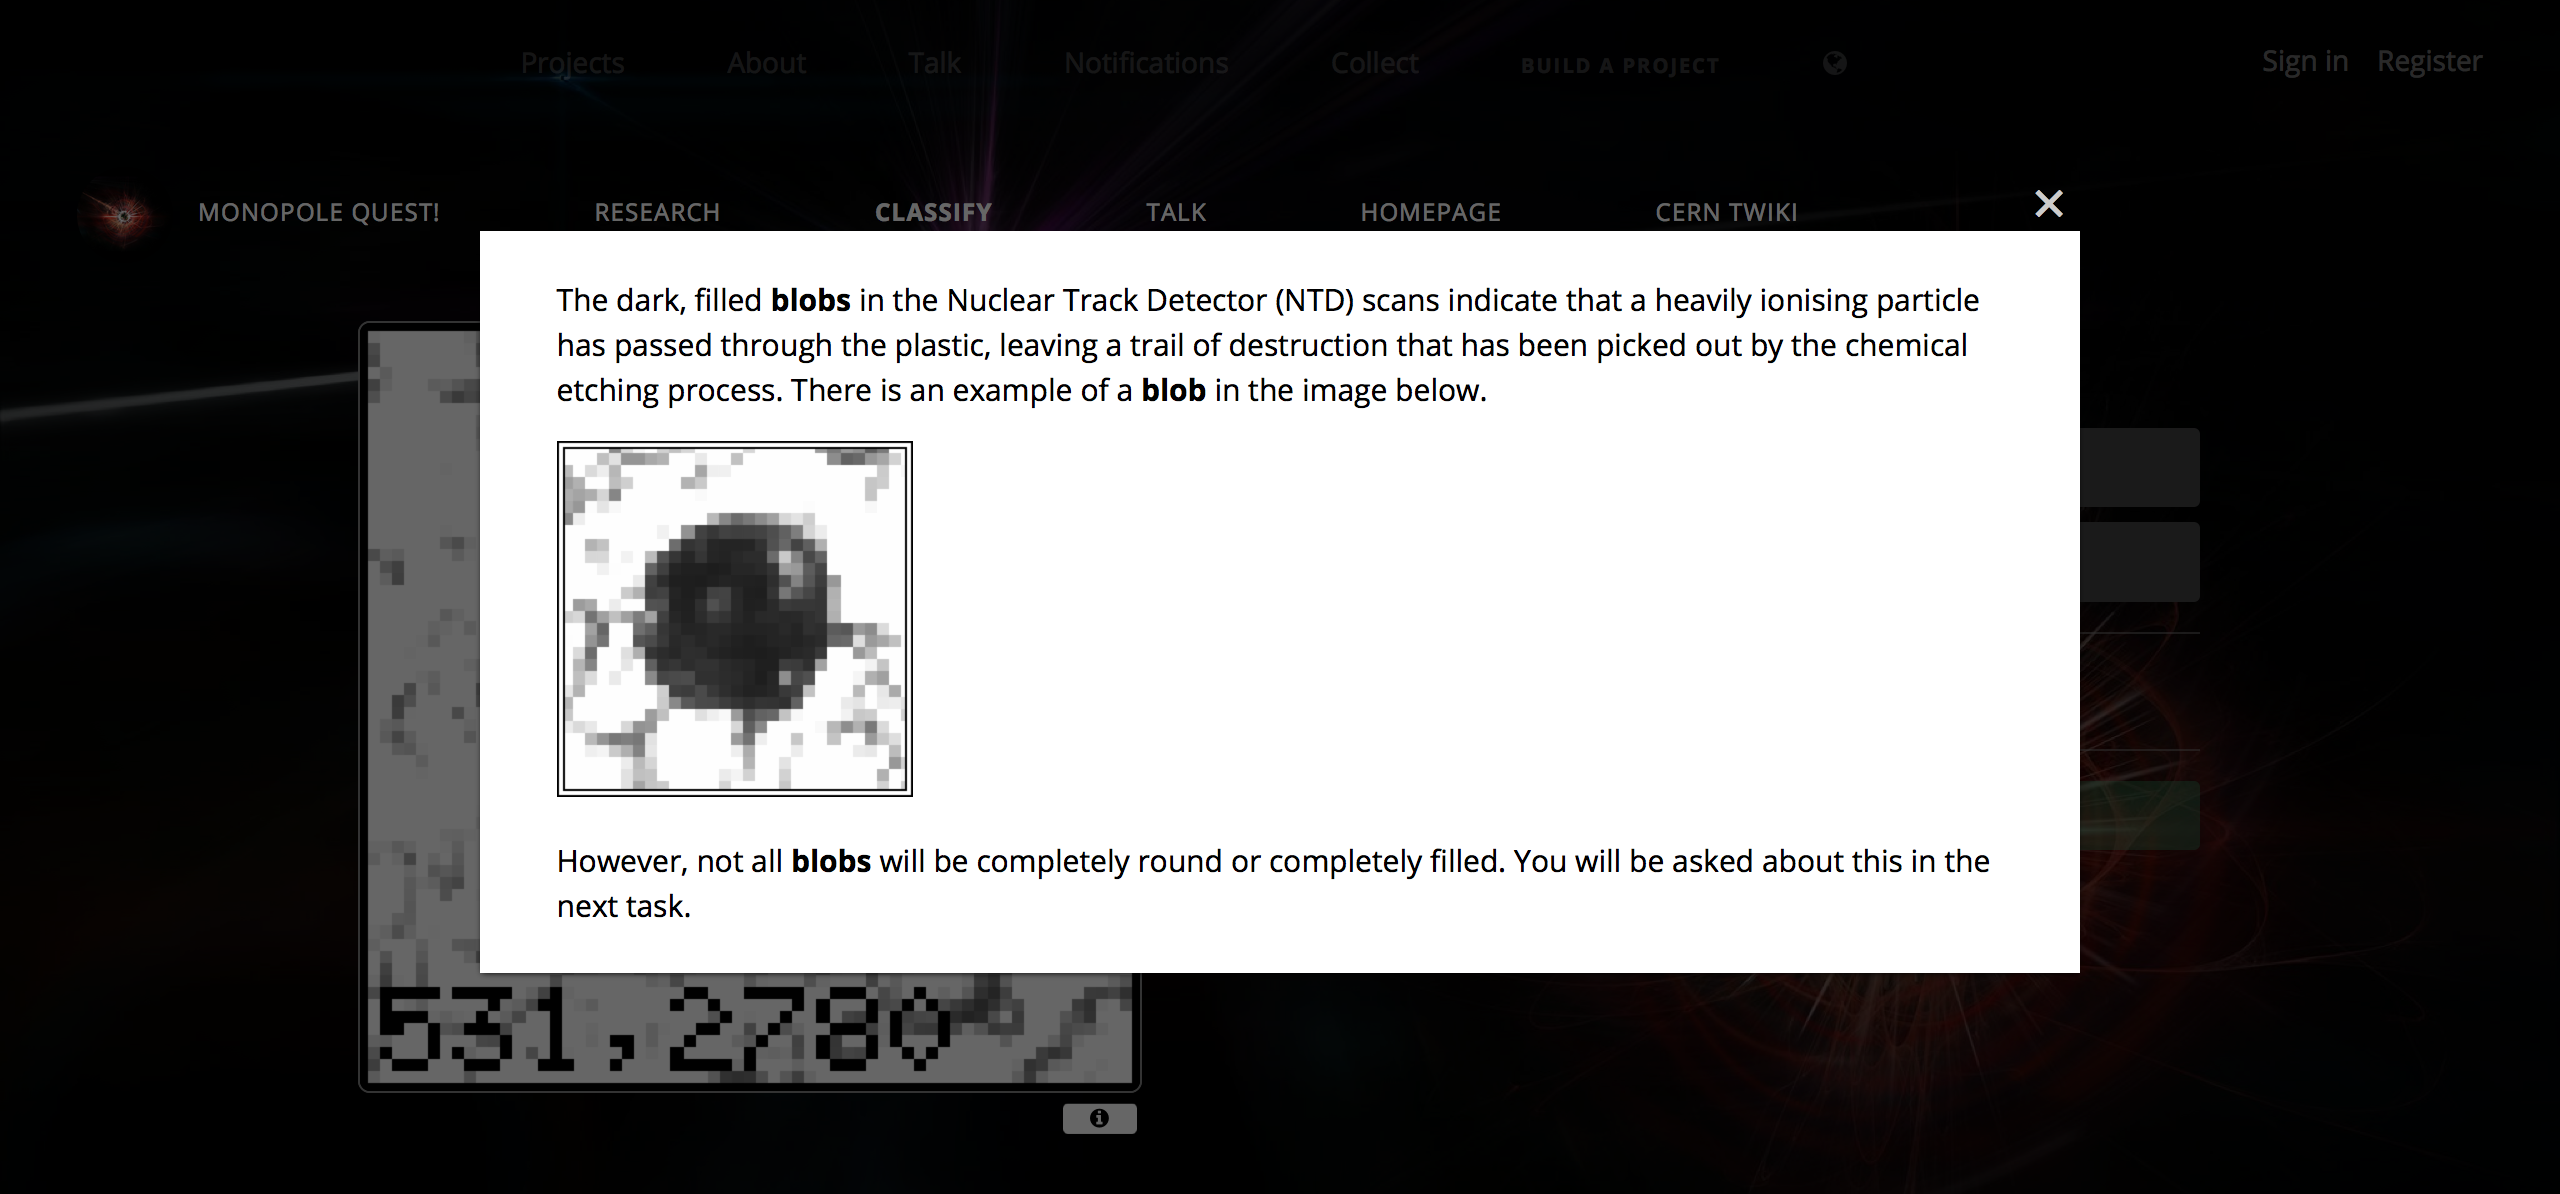
\includegraphics[width=0.8\textwidth]{assets/images/mqhelp/mqhelp.png}
  \caption[Monopole Quest! An example help message]
  {\label{fig:mqhelp}An example help pop-up message in Monopole Quest! (Jan. 2017).}
\end{figure}
%

\clearpage

%-----------------------------------------------------------------------------
\subsubsection{What am I looking at?}
\label{sec:mqlookingat}
%-----------------------------------------------------------------------------
The data used in Monopole Quest! comes from scans of plastic from the
\ac{MoEDAL} \acp{NTD}.
All of it is real data from the experiment,
but some images were made using plastic exposed to different environments
and scanned in different laboratories:

\begin{enumerate}
\item Some plastic was exposed to LHC collisions at 8 TeV centre-of-mass energy;
\item Some plastic was exposed to LHC collisions at 13 TeV centre-of mass energy;
\item Some plastic was exposed to a heavy ion test beam
(see Figure~\ref{fig:bnltestbeam});
\item Some plastic was exposed to both LHC collisions and a heavy ion test beam.
\end{enumerate}

%
\begin{figure}[htbp]
  \centering
  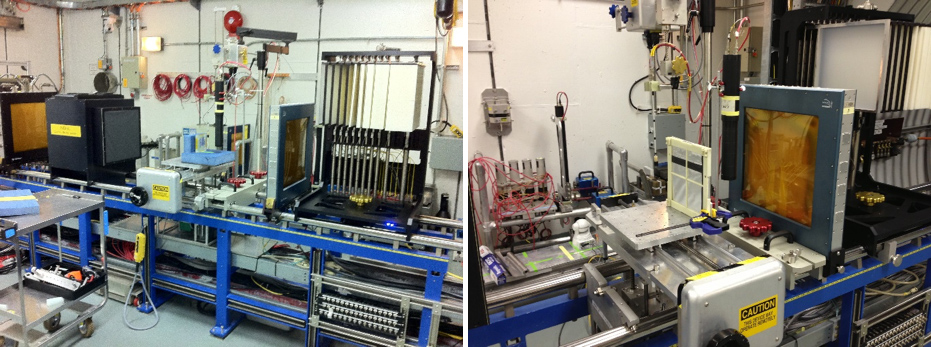
\includegraphics[width=1.0\textwidth]{assets/images/bnltestbeam/bnltestbeam.jpg}
  \caption[MoEDAL NTD samples in the BNL test beam]
  {\label{fig:bnltestbeam}\ac{MoEDAL} \ac{NTD} samples being exposed to a
heavy ion test beam at the \ac{NASA} \acf{SRL}, \acf{BNL}.
Exposing \ac{NTD} plastic to heavy ions from test beams allows us to see
what monopole-like signals might look like and put our analysis procedures
through their paces.  %
Image credit: R. Soluk/the MoEDAL Collaboration; %
please contact them regarding licensing/re-use of this image.}
\end{figure}
%

Analysis of plastic exposed to these different conditions is necessary to
provide control samples and to test our analysis procedures
(including Monopole Quest!) with monopole-like signals from the heavy ions.
As a Zooniverse volunteer, we won’t tell you which sample type you are 
looking at (as this might bias your answers).
However, all data and classifications are useful to the \ac{MoEDAL}
science programme, so please do as many as you can!

%-----------------------------------------------------------------------------
\subsubsection{What happens next? Continuing your MoEDAL journey}
\label{sec:mqnext}
%-----------------------------------------------------------------------------
Your classifications are stored by Monopole Quest! for further analysis
by the \ac{MoEDAL} science team -- which could include you!
As you and your school get further involved with \ac{IRIS},
data based on the user classifications (including yours) can be made 
available for individual or group research projects.
Contact the \ac{IRIS} team with your Zooniverse usernames
(so we can verify how many classifications you have made)
and project ideas to find out more.
Then, as with all \ac{IRIS} research,
the aim is to publish results based on the data and analysis in
peer-reviewed scientific journals.
You can see the many examples of Zooniverse-powered publications on their
website -- and with the support of CERN@school through IRIS
and the MoEDAL Collaboration, you should be able to add to this.

{\color{white}Spacer}
\\[1cm]

\begin{center}
\textbf{What can {\em you} do with \ac{MoEDAL} and \ac{IRIS}?}
\end{center}


\clearpage

%
%%%%%%%%%%%%%%%%%%%%%%%%%%%%%%%%%%%%%%%%%%%%%%%%%%%%%%%%%%%%%%%%%%%%%%%%%%%%%%%
% Bibliography
%%%%%%%%%%%%%%%%%%%%%%%%%%%%%%%%%%%%%%%%%%%%%%%%%%%%%%%%%%%%%%%%%%%%%%%%%%%%%%%
%
\section{References}
\bibliographystyle{unsrt.bst}
\bibliography{MoEDAL}
%
%------------------------------------------------------------------------------

\clearpage

%%%%%%%%%%%%%%%%%%%%%%%%%%%%%%%%%%%%%%%%%%%%%%%%%%%%%%%%%%%%%%%%%%%%%%%%%%%%%%
\section{Acronyms}
\label{sec:acronyms}
%%%%%%%%%%%%%%%%%%%%%%%%%%%%%%%%%%%%%%%%%%%%%%%%%%%%%%%%%%%%%%%%%%%%%%%%%%%%%%

\begin{acronym}
\acro{ALICE}{A Large Ion Collider Experiment}
\acro{AMANDA}{Antarctic Muon and Neutrino Detector Array}
\acro{ANTARES}{Astronomy with a Neutrino Telescope and Abyss environmental RESearch project}
\acro{ATLAS}{A Toroidal LHC ApparatuS}
\acro{BNL}{Brookhaven National Laboratory}
\acro{BSM}{Beyond Standard Model\acroextra{ (physics)}}
\acro{CDF}{Collider Detector at Fermilab}
\acro{CERN}{Organisation Europ\'een pour la Recherche Nucl\'aire}
\acro{CMS}{\acroextra{The }Compact Muon Solenoid experiment}
\acro{DESY}{Deutsches Elektronen-SYnchrotron\acroextra{ (Germany)}}
\acro{GUT}{Grand Unified Theory}
\acro{HERA}{Hadron- Elektron-Ring-Anlage\acroextra{ (Hadron Electron Ring Facility)}}
\acro{HIP}{Highly Ionising Particle}
\acro{IRIS}{\acroextra{The }Institute for Research in Schools}
\acro{ISS}{International Space Station}
\acro{KEK}{\acroextra{The }High Energy Accelerator Organisation\acroextra{ (Japan)}}
\acro{LEP}{Large Electron-Positron\acroextra{ collider}}
\acro{LHC}{Large Hadron Collider}
\acro{LHCb}{\acroextra{The }Large Hadron Collider Beauty\acroextra{ experiment}}
\acro{MACRO}{Monopole, Astrophysics and Cosmic Ray\acroextra{ observatory (Italy)}}
\acro{MMT}{Magnetic Monopole Trapper}
\acro{MODAL}{MOnopole Detector at LEP}
\acro{MoEDAL}{Monopole and Exotics Detector at the LHC}
\acro{NASA}{National Aeronautics and Space Administration\acroextra{ (US)}}
\acro{NTD}{Nuclear Track Detector}
\acro{OPAL}{Omni-Purpose Apparatus at LEP}
\acro{PEP}{Positron Electron Project\acroextra{ (SLAC, US)}}
\acro{QFT}{Quantum Field Theory}
\acro{SLAC}{Stanford Linear Accelerator Center\acroextra{ (US)}}
\acro{SLIM}{Search for LIght magnetic Monopoles\acroextra{ experiment}}
\acro{SQUID}{Superconducting QUantum Interference Device}
\acro{SRL}{\acroextra{The NASA }Space Radiation Laboratory\acroextra{ (US)}}
\acro{TDR}{Technical Design Report\acroextra{ for, e.g. the MoEDAL experiment}}
\acro{TeV}{tera-electron volts}
\acro{VeLo}{Vertex Locator\acroextra{ (LHCb subdetector system)}}
\acro{VHCC}{Very High Charge Catcher}
\end{acronym}


\clearpage


%%%%%%%%%%%%%%%%%%%%%%%%%%%%%%%%%%%%%%%%%%%%%%%%%%%%%%%%%%%%%%%%%%%%%%%%%%%%%%%
\section{Acknowledgements}
\label{sec:ack}
%%%%%%%%%%%%%%%%%%%%%%%%%%%%%%%%%%%%%%%%%%%%%%%%%%%%%%%%%%%%%%%%%%%%%%%%%%%%%%%
This work was supported by the 
UK Science and Technology Facilities Council (STFC) 
via grant numbers 
ST/J000256/1 
and 
ST/N00101X/1,
as well as a Special Award from the Royal Commission for the Exhibition of 1851.
%
Computing resource and expertise was kindly provided by
the UK's GridPP Collaboration~\cite{gridpp2006,gridpp2009}\footnote{
\href{http://www.gridpp.ac.uk}{http://www.gridpp.ac.uk}}.


%%%%%%%%%%%%%%%%%%%%%%%%%%%%%%%%%%%%%%%%%%%%%%%%%%%%%%%%%%%%%%%%%%%%%%%%%%%%%%%
\section*{Version History}
%%%%%%%%%%%%%%%%%%%%%%%%%%%%%%%%%%%%%%%%%%%%%%%%%%%%%%%%%%%%%%%%%%%%%%%%%%%%%%%
%______________________________________________________________________________
\begin{table}[h]
\caption[Document version history]{\label{tab:version}Version history.}
\lineup
\begin{indented}
\item[]\begin{tabular}{@{}cllc}
\br
\centre{1}{$\quad$Version    $\quad$} & 
\centre{1}{$\quad$DOI        $\quad$} & 
\centre{1}{$\quad$Description$\quad$} &
\centre{1}{$\quad$Author     $\quad$} \\
\mr
1.0 & \href{http://doi.org/10.5281/zenodo.248615}{10.5281/zenodo.248615} & Initial version. & TW \\
\br
\end{tabular}
\end{indented}
\end{table}
%______________________________________________________________________________

\end{document}
